\begin{ex} %[3P1Y1-1][Loai1] 
(QG - 2015) Một vật nhỏ dao động theo phương trình $x=5\cos \left(\omega t+0,5\pi\right)\ cm$. Pha ban đầu của dao động là
\choice
{$\pi$}
{\True $0,5 \pi$}
{$0,25\pi$}
{$1,5 \pi$}
\loigiai{
Ta có: $x = A\cos\left(\omega t + \varphi \right) = 5\cos\left(\omega t + 0,5\pi \right)\ cm\Rightarrow$ pha ban đầu $\varphi  = 0,5\pi\ rad$.
}
%\haidong{3}
\end{ex} \haidong{15}
\begin{ex}%[3P1Y1-2][Loai1]
Một chất điểm dao động theo phương trình $x = 6\cos \omega t$ cm. Dao động của chất điểm có biên độ là
\choice
{\True 6 cm}
{3 cm}
{2 cm}
{12 cm}
\loigiai{
Phương trình dao động tổng hợp là: $x = A\cos \omega t$ cm $\Rightarrow$ $A = 6$ cm.
}
%\haidong{2}
\end{ex} \haidong{15}
\begin{ex}%book
Một chất điểm dao động điều hòa với phương trình $x=2 \cos 4 \pi t\ cm$. Chu kì dao động của chất điểm bằng bao nhiêu giây?
\shortans[oly]{0,5}
\loigiai{
$T=\dfrac{2 \pi}{\omega}=\dfrac{2 \pi}{4 \pi}=0,5 \ s$
}
%\haidong{2}
\end{ex} \haidong{15}
\begin{ex}%book
\immini[thm]{
Xác định biên độ, chu kì, tần số, tần số góc của mỗi dao động có đồ thị li độ - thời gian như hình vẽ.
}{\begin{tikzpicture}[scale=0.5,transform shape]
%Hệ trục toạ độ
\tkzDefPoints{0/0/x', 10/0/x, 0/-2.2/y', 0/2.3/y}
\tkzDrawSegments[->,add = 0 and .05](x',x)
\tkzDrawSegments[->,add = 0 and .05](y',y)
\tkzLabelPoint[below right](x){$t\ (s)$}
\tkzLabelPoint[above=10pt](y){$x\ (m)$}
%Lưới
\draw  [help  lines, xstep=2cm,ystep=0.5cm]  (x' |- y')  grid  (x |- y);
%Chia khoảng trên trục x, y
\foreach  \x  in  {2,4,...,10}
{\draw[thin]  (\x,-0.1)  --  (\x,0.1);}
\foreach  \y  in  {-2,-1,1,2}
{\draw[thin]  (-0.1,\y)  --  (0.1,\y);}
%Đánh số toạ độ
\pgfkeys{/pgf/number format/use comma}
\foreach \x[evaluate=\x as \text using \x*0.01] in {2,4,...,10}{
\node[below=3pt] at (\x,-2){\pgfmathprintnumber[fixed,fixed zerofill,precision=2]{\text}};}
\foreach \y[evaluate=\y as \text using \y*0.1] in {-2,-1,1,2}{
\node[left=3pt] at (0,\y){\pgfmathprintnumber[fixed,fixed zerofill,precision=1]{\text}};}
\node[below left] at (0,0){$O$};
%Đồ thị xanh
\def\A{1.5} % Biên độ
\def\T{5} % Chu kì
\def\Phi{90} % Pha ban đầu
{\draw [blue,dashed, line width = 1.2pt, domain=0:10, samples=500]%
plot (\x, {(\A)*cos(360/\T*\x+\Phi)});}
%Đồ thị đỏ
\def\A{2} % Biên độ
\def\T{5} % Chu kì
\def\Phi{35} % Pha ban đầu
{\draw [red, line width = 1.2pt, domain=0:10, samples=500]%
plot (\x, {(\A)*cos(360/\T*\x+\Phi)});}
\end{tikzpicture}}
\loigiai{
\begin{itemize}
\item Biên độ: $A_1=20\ cm;\ A_2=15\ cm$. Chu kì: $T_1=T_2=0,05\ s$
\item Tần số: $f_1=f_2=20\ Hz$. Tần số góc: $\omega_1=\omega_2=40\pi\ rad/s$.
\end{itemize}
}
%\haidong{4}
\end{ex} \haidong{15}
\section{VẬN TỐC GIA TỐC}
\begin{ex}%[3P1B2-1][Loai1]
Một vật dao động điều hòa với biên độ A và tần số góc $\omega$. Tốc độ cực đại của vật dao động là
\choice
{\True $v_{\max} = \omega A$}
{$v_{\max} = \omega^2A$}
{$v_{\max} = \omega A^2$}
{$v_{\max} = \omega^2A^2$}
\loigiai{
Tốc độ cực đại của vật dao động là: $v_{\max} = \omega A$.
}
\end{ex} \haidong{15}
\begin{ex} %[3P1Y2-1][Loai1] 
(QG - 2018) Một vật dao động điều hòa trên trục Ox. Vận tốc của vật
\choice
{luôn có giá trị không đổi}
{luôn có giá trị dương}
{là hàm bậc hai của thời gian}
{\True biến thiên điều hòa theo thời gian}
\loigiai{
Vận tốc của vật biến thiên điều hòa theo thời gian.
}
\end{ex} \haidong{15}
\begin{ex}%[3P1Y2-1][Loai1]
Một vật dao động điều hòa với biên độ A, tần số góc $\omega$. Gia tốc của vật trong quá trình vật dao động có độ lớn cực tiểu là
\choice
{\True 0}
{$-m\omega^2A$}
{$- \omega A$}
{$-\omega^2A$}
\loigiai{
Gia tốc của vật trong quá trình vật dao động có độ lớn cực tiểu là 0.
}
\end{ex} \haidong{15}
\begin{ex}%[3P1B2-1][Loai1]
Một vật dao động điều hòa với biên độ A và tần số góc $\omega$. Gia tốc cực đại của vật dao động là
\choice
{$a_{\max} = \omega A$}
{\True $a_{\max} = \omega^2A$}
{$a_{\max} = \omega A^2$}
{$a_{\max} = \omega^2A^2$}
\loigiai{
Gia tốc cực đại của vật dao động là: $a_{\max} = \omega^2A$.
}
\end{ex} \haidong{15}
\begin{ex}%[3P1B2-1][Loai1]
Một vật dao động điều hòa với biên độ A và tốc độ cực đại $v_{\max}$. Tần số góc của vật dao động là
\choice
{\True $\dfrac{v_{\max}}{A}$}
{$\dfrac{v_{\max}}{\pi A}$}
{$\dfrac{v_{\max}}{2\pi A}$}
{$\dfrac{v_{\max}}{2A}$}
\loigiai{
Tần số góc của vật dao động là: $\dfrac{v_{\max}}{A}$.
}
\end{ex} \haidong{15}

\begin{ex}%book
Phát biểu nào sau đây \textbf{sai} về gia tốc của một vật dao động điều hoà?
\choice
{Gia tốc đổi chiều khi vật đi qua vị trí cân bằng}
{\True Gia tốc luôn ngược chiều với vận tốc}
{Gia tốc luôn hướng về vị trí cân bằng}
{Gia tốc biến đổi ngược pha với li độ}
\end{ex} \haidong{15}
\begin{ex}%book %[3P1B2-1][Loai1] 
(QG - 2018) Một vật dao động điều hòa trên trục Ox quanh vị trí cân bằng O. Khi nói về gia tốc của vật, phát biểu nào sau đây \textbf{sai}?
\choice
{Gia tốc có độ lớn tỉ lệ với độ lớn li độ của vật}
{\True Vectơ gia tốc luôn cùng hướng với vectơ vận tốc}
{Vectơ gia tốc luôn hướng về vị trí cân bằng}
{Gia tốc luôn ngược dấu với li độ của vật}
\loigiai{
Gia tốc của vật trong dao động điều hòa tỉ lệ với độ lớn li độ của vật, luôn hướng về vị trí cân bằng, luôn ngược dấu với li độ của vật. (A, C và D đúng).
}
\end{ex} \haidong{15} 
\begin{ex}%book%[3P1Y2-1][Loai1]
Một chất điểm dao động điều hoà trên trục Ox. Khi đi từ vị trí biên âm tới biên dương thì
\choice
{\True vận tốc của vật có giá trị tăng từ 0 lên cực đại ($\omega A$) rồi giảm về 0}
{tốc độ của vật tăng lên}
{vận tốc có giá trị âm}
{gia tốc của vật có giá trị tăng từ cực tiểu ($- \omega^2A$) lên cực đại ($\omega^2A$)}
\loigiai{
Khi đi từ vị trí biên âm tới biên dương thì vận tốc của vật có giá trị tăng từ 0 lên cực đại ($\omega A$) rồi giảm về 0.
}
\end{ex} \haidong{15}

\begin{ex}%book
Cho các nhận định sau về một chất điểm đang dao động điều hòa.
\choiceTF[t]
{Một chất điểm dao động điều hòa, khi đi từ vị trí biên dương về vị trí biên âm thì gia tốc luôn giảm}
{\True Tại thời điểm $t$, vận tốc của chất điểm đang giảm thì khi đó gia tốc dương}
{Tại thời điểm $t$, khi đi từ vị trí biên dương về vị trí biên âm thì tốc độ luôn giảm}
{\True Tại thời điểm $t$, gia tốc của chất điểm đang tăng thì khi đó vận tốc âm}
\loigiai{
\begin{itemchoice}
\itemch
\itemch
\itemch
\itemch
\end{itemchoice}
}
\end{ex} \haidong{15}
\begin{ex}%book
Cho các nhận định sau về một chất điểm đang dao động điều hòa.
\choiceTF[t]
{Chuyển động của vật từ vị trí biên về vị trí cân bằng là chuyển động nhanh dần}
{\True Khi đi từ vị trí cân bằng ra biên dương là chuyển động chậm dần}
{\True Khi đi từ vị trí cân bằng ra biên âm là chuyển động chậm dần}
{Khi vật chuyển động nhanh dần theo chiều dương thì vật có li độ dương và vận tốc âm} \loigiai{
\begin{itemchoice}
\itemch
\itemch
\itemch
\itemch
\end{itemchoice}
}
\end{ex} \haidong{15}
\begin{ex}%book
Một chất điểm chuyển động tròn đều trên một đường tròn với tốc độ dài 160 cm/s và tốc độ góc 4 rad/s. Hình chiếu P của chất điểm M trên một đường thẳng cố định nằm trong mặt phẳng hình tròn dao động điều hoà với biên độ và chu kì lần lượt là
\choice
{$40\ cm;\ 0,25\ s$}
{\True $40\ cm;\ 1,57\ s$}
{$40\ m;\ 0,25\ s$}
{$2,5\ m;\ 0,25\ s$}
%\haidong{3}
\end{ex} \haidong{15}


\section{Pha và trạng thái dao động}
%\loai{Cho pha, tìm li độ và chiều}
\begin{ex}%book%[3P1-4.1B][Loai1]
Một vật nhỏ dao động điều hòa với biên độ A. Khi pha dao động của vật (pha của li độ x) là  $-\dfrac{\pi}{3}$  thì vật
\choice
{đi qua vị trí có li độ 0,5A theo chiều âm}
{\True đi qua vị trí có li độ 0,5A theo chiều dương}
{đi qua vị trí có li độ $- 0,5A$ theo chiều âm}
{đi qua vị trí có li độ $- 0,5A$ theo chiều dương}
\loigiai{
Ta có: ${\phi _x} = - \dfrac{\pi}{3} \Rightarrow x = \dfrac{A}{2}\ ( + )$.
}
%\haidong{3}
\end{ex} \haidong{15}
%\loai{Tìm trạng thái dao động tại thời điểm t}
\begin{ex}%book%[3P1-4.1K][Loai1]
Một vật dao động điều hoà trên trục Ox với phương trình  $x=4\cos \left( 2\pi t+\dfrac{\pi}{3} \right)$ cm. Lấy  $\pi ^2  = 10$. Tại thời điểm 3,5 s thì
\choice
{$x = 2$ cm đang giảm}
{$v =  4\pi \sqrt{3}$ cm/s đang giảm}
{$a =  -0,8\sqrt{2}$  $m/s^2$ đang tăng}
{\True $x = - 2$ cm đang tăng}
\loigiai{
\begin{itemize}
\item Pha dao động tại thời điểm 3,5 s: $\phi=2\pi.3,5+\dfrac{\pi}{3}=\dfrac{22\pi}{3}=\dfrac{24\pi}{3}-\dfrac{2\pi}{3}$.
\item Dựa vào đường tròn pha ta có $x = - 2$ cm đang tăng, $v =  4\pi \sqrt{3}$ cm/s đang tăng.
\item Gia tốc $a=-\omega^2.x= 0,8\ m/s^2$.
\item Do x đang tăng nên a đang giảm.
\end{itemize}
}
%\haidong{4}
\end{ex} \haidong{15}
%\loai{Cho trạng thái của x, tìm trạng thái của v}
\begin{ex}%book%[3P1-4.1B][Loai1]
Một vật nhỏ dao động điều hòa trên trục Ox với biên độ A và tần số góc $\omega$. Khi vật đi qua $-0,5A$ theo chiều âm thì vận tốc của vật có giá trị
\choice
{$\dfrac{\omega A\sqrt{3}}{2}$ và đang tăng}
{\True $-\dfrac{\omega A\sqrt{3}}{2}$  và đang tăng}
{$-\dfrac{\omega A\sqrt{3}}{2}$  và đang giảm}
{$0,5\omega A$ và đang giảm}
\loigiai{
Khi $x =  -\dfrac{A}{2}(-)$: $\phi_{x}=\dfrac{2\pi}{3}\Rightarrow \phi_{v}=\phi_{x}+\dfrac{\pi}{2}=\dfrac{7\pi}{6}\equiv -\dfrac{5\pi}{6}\Rightarrow v=-\dfrac{{{v}_{\max }}\sqrt{3}}{2}\ (+)$.
}
%\haidong{5}
\end{ex} \haidong{15}
%\loai{Cho pha, trạng thái dao động tìm đại lượng khác}
\begin{ex}%book %[3P1-4.1B][Loai1] 
Một vật dao động điều hoà trên đoạn thẳng dài 10 cm. Khi pha dao động bằng $\dfrac{\pi}{3}$ thì vật có vận tốc $v = -5\pi \sqrt{3}$ cm/s. Khi qua vị trí cân bằng vật có vận tốc là
\choice 
{5$\pi$ cm/s}
{\True 10$\pi$ cm/s}
{20$\pi$ cm/s}
{15$\pi$ cm/s}
\loigiai{
Vật dao động trên đoạn thẳng dài 10 cm nên $A = 5\ cm;\ \varphi = \dfrac{\pi}{3}\Rightarrow x = \dfrac{A}{2}\Rightarrow v = -\dfrac{\sqrt3}{2}v_{\max} \Rightarrow v_{\max} = 10\pi\ cm/s$.
}
%\haidong{5}
\end{ex} \haidong{15}
%\loai{Tính độ lệch pha}
\begin{ex}%book %[3P1-4.1B][Loai1] 
\nguon{QG - 2016} Cho hai dao động điều hòa cùng phương, có phương trình lần lượt là $x_1=10\cos\left(100\pi t-0,5\pi\right)\ cm$, $x_2=10\cos\left(100\pi t+0,5\pi\right)\ cm $. Độ lệch pha của hai dao động này có độ lớn là
\choice
{0}
{$0,25\pi$}
{\True $\pi$}
{$0,5\pi$}
\loigiai{
Hai dao động đã cho ngược pha nhau.
}
%\haidong{4}
\end{ex} \haidong{15}
%\loai{So sánh pha của hai dao động}
\begin{ex}%book %[3P1-4.1K][Loai1]  
Cho hai chất điểm dao động điều hòa cùng phương với phương trình lần lượt như sau: $x_1 = 5\cos\left(8t + \dfrac{\pi}{6}\right)$ cm, $x_2 = 6\sin\left(8t + \dfrac{\pi}{2}\right)$ cm. Kết luận nào sau đây là đúng?
\choice
{Dao động thứ nhất trễ pha hơn dao động thứ hai góc $\dfrac{\pi}{3}$}
{\True Dao động thứ nhất sớm pha hơn dao động thứ hai góc $\dfrac{\pi}{6}$}
{Dao động thứ nhất trễ pha hơn dao động thứ hai góc $\dfrac{5\pi}{6}$}
{Dao động thứ nhất sớm pha hơn dao động thứ hai góc $\dfrac{\pi}{3}$}
\loigiai{
\begin{itemize}
\item Ta có: $x_1 = 5\cos\left(8 t+ \dfrac{\pi}{6}\right);\ x_2 = 6\cos 8 t$.
\item Dao động thứ nhất sớm pha hơn dao động thứ hai góc $\dfrac{\pi}{6}$.
\end{itemize}}
%\haidong{3}
\end{ex} \haidong{15}
\begin{ex}%book %[3P1B4-1][Loai1]  
Biết pha ban đầu của một vật dao động điều hòa, ta xác định được
\choice
{quỹ đạo dao động}
{cách kích thích dao động}
{chu kì và trạng thái dao động}
{\True chiều chuyển động của vật lúc ban đầu}
\loigiai{
Pha dao động cho ta biết trạng thái chuyển động của vật.
}
\end{ex} \haidong{15}
%\loai{Cho li độ. Tìm pha dao động}
\begin{ex}%book%[3P1K4-1][Loai1]
Cho một chất điểm đang dao động điều hòa với biên độ A. Biết tại thời điểm ban đầu $\left(t = 0\right)$ chất điểm đi qua vị trí có li độ $\dfrac{A}{2}$ và đang chuyển động theo chiều dương của trục tọa độ. Pha ban đầu của dao động là
\choice 
{$\dfrac{\pi}{4}$ rad}
{$\dfrac{\pi}{6}$ rad}
{$\dfrac{\pi}{3}$ rad}
{\True $-\dfrac{\pi}{3}$ rad}
\loigiai{
Sử dụng đường tròn lượng giác ta suy ra được pha của dao động là $-\dfrac{\pi}{3}$.
}
%\haidong{3}
\end{ex} \haidong{15}
 
%\loai{Cho pha, tìm li độ và chiều}
\begin{ex}%book%[3P1B4-1][Loai1]
Một vật nhỏ dao động điều hòa với biên độ A trên trục Ox. Khi pha của vận tốc là 0 thì vật
\choice
{ở biên dương $x = A$}
{đi qua vị trí cân bằng theo chiều âm}
{\True đi qua vị trí cân bằng theo chiều dương}
{ở biên âm $x = -A$}
\loigiai{
Ta có: $\phi _x=\phi _v-\dfrac{\pi}{2} = - \dfrac{\pi}{2} \Rightarrow x = 0\quad (+)$.
}
%\haidong{3}
\end{ex} \haidong{15}
\begin{ex}%book%[3P1K4-1][Loai1] 
Phương trình của một dao động điều hoà của một chất điểm có dạng $x = 6\sin\left(10\pi t + \dfrac{\pi}{6}\right)$ cm. Khi pha dao động bằng $-\dfrac{\pi}{4}$ thì vị trí của chất điểm là
\choice
{$x = \sqrt{2}$ cm}
{\True $x = 3\sqrt{2}$ cm}
{$x = 3$ cm}
{$x = 6$ cm}
\loigiai{
\begin{itemize}
\item Ta có: $x = 6\sin\left(10\pi t+ \dfrac{\pi}{6}\right) = 6\cos\left(10\pi t- \dfrac{\pi}{3}\right)$.
\item Khi pha dao động bằng $-\dfrac{\pi}{4}$ thì $x = 6\cos\left(-\dfrac{\pi}{4}\right) = 3\sqrt{2}$ cm.
\end{itemize}
}
%\haidong{3}
\end{ex} \haidong{15}

%\loai{Cho pha, tìm vận tốc hoặc gia tốc}
\begin{ex}%book%[3P1B4-1][Loai1]
Một vật nhỏ dao động điều hòa trên trục Ox với vận tốc có giá trị cực đại là $v_{\max}$. Khi pha dao động của vật (pha của li độ x) là  $-\dfrac{\pi}{3}$  thì vận tốc có giá trị
\choice
{$0,5v_{\max}$ và đang giảm}
{$0$ và đang tăng}
{$0,5v_{\max}$ và đang tăng}
{\True $\dfrac{{{v}_{\max }}\sqrt{3}}{2}$ và đang giảm}
\loigiai{
Ta có: $\phi_v=\phi_x+\dfrac{\pi}{2}=-\dfrac{\pi}{3}+\dfrac{\pi}{2}=\dfrac{\pi}{6}\Rightarrow v=\dfrac{v_{\max}\sqrt{3}}{2}\quad (-)$.
}
%\haidong{3}
\end{ex} \haidong{15}
\begin{ex}%book %[3P1B4-1][Loai1]  
Một con lắc lò xo dao động theo phương ngang với chiều dài quỹ đạo là 14 cm, tần số góc $\omega =2\pi \ rad/s$. Tốc độ của vật khi pha dao động bằng $\dfrac{\pi }{3}$ rad là
\choice
{$\dfrac{{7\pi }}{{\sqrt{3}}}$ cm/s}
{\True $7\pi \sqrt{3}$ cm/s}
{$7\pi $ cm/s}
{$7\pi \sqrt{2}$ cm/s}
\loigiai{
\begin{itemize}
\item Biên độ dao động của vật: $A=0,5L=7$ cm.
\item Tốc độ của vật: $\left|v\right|=A\omega \sin \varphi =7\pi \sqrt{3}$ cm/s.
\end{itemize}
}
%\haidong{3}
\end{ex} \haidong{15}
%\loai{Xác định trạng thái tại thời điểm $t=0$}
\begin{ex}%book%[3P1B4-1][Loai1]
Phương trình dao động của một vật là $x=5\sin \left(\omega t-\dfrac{5\pi}{6}\right)$ cm. Gốc thời gian $t = 0$ được chọn là lúc
\choice
{\True vật có li độ $- 2,5\ cm$, đang chuyển động ra phía biên}
{vật có li độ $2,5\ cm$, đang chuyển động về phía vị trí cân bằng}
{vật có li độ $-2,5\ cm$, đang chuyển động về phía vị trí cân bằng}
{vật có li độ $2,5\ cm$, đang chuyển động về phía biên}
\loigiai{
\begin{itemize}
\item Ta có:  $x=5\sin \left(\omega t-\dfrac{5\pi}{6}\right)=5\cos \left(\omega t-\dfrac{4\pi}{3}\right)=5\cos \left(\omega t+\dfrac{2\pi}{3}\right)$ cm.
\item Taị $t = 0$, pha dao động là $\phi  = \dfrac{2\pi}{3} \Leftrightarrow $ vật có li độ $x=-\dfrac{A}{2}=-2,5\ cm$ và đang đi ra biên.
\end{itemize}
}
%\haidong{4}
\end{ex} \haidong{15}

%\loai{Tìm trạng thái dao động tại thời điểm t}
\begin{ex}%book%[3P1B4-1][Loai1]
Một chất điểm dao động điều hòa trên trục Ox có phương trình $x=10\sin \left(2\pi t+\dfrac{\pi}{3}\right)$ (x tính bằng cm, t tính bằng s) thì thời điểm $t = 2,5$ s vật
\choice
{\True đi qua vị trí có li độ $x=-5\sqrt{3}$ cm và đang chuyển động theo chiều âm trục Ox}
{đi qua vị trí có li độ $x=-5\sqrt{3}$ cm và đang chuyển động theo chiều dương trục Ox}
{đi qua vị trí có li độ $x = - 5$ cm và đang chuyển động theo chiều dương trục Ox}
{đi qua vị trí có li độ $x = - 5$ cm và đang chuyển động theo chiều âm của trục Ox}
\loigiai{
\begin{itemize}
\item Đưa phương trình dao động về dạng chuẩn tắc: $x=10 \cos\left(2\pi t-\dfrac{\pi}{6}\right)$ cm. 
\item Pha dao động của vật tại $t = 2,5$ s là: $\phi_{2,5\ s}=2\pi .2,5-\dfrac{\pi}{6}=\dfrac{29\pi}{6}\equiv \dfrac{5\pi}{6}\Leftrightarrow  x=-\dfrac{A\sqrt{3}}{2}=-5\sqrt{3}$ cm $(-)$.
\end{itemize}
}
%\haidong{3}
\end{ex} \haidong{15}
%\loai{Cho trạng thái của x, tìm trạng thái của v}
\begin{ex}%book%[3P1B4-1][Loai1]
Một vật nhỏ dao động điều hòa trên trục Ox với biên độ A và tần số góc $\omega$. Khi vật có vận tốc $-0,5\omega A$ và đang có xu hướng giảm thì trạng thái dao động của vật là
\choice
{Vật đi qua li độ  $\dfrac{A\sqrt{3}}{2}$ theo chiều dương}
{\True Vật đi qua li độ  $\dfrac{A\sqrt{3}}{2}$ theo chiều âm}
{Vật đi qua li độ  $-\dfrac{A\sqrt{3}}{2}$ theo chiều âm}
{Vật qua li độ $0,5A$ theo chiều âm}
\loigiai{
Khi $x =  -\dfrac{v_{\max}}{2}\ (-):\ \phi_v=\dfrac{2\pi}{3}
\Rightarrow \phi_x=\phi_v-\dfrac{\pi}{2}=\dfrac{\pi}{6}\Rightarrow x=\dfrac{A\sqrt{3}}{2}\ (-)$.
}
%\haidong{4}
\end{ex} \haidong{15}
%\loai{Cho pha, trạng thái dao động tìm đại lượng khác}
%\loai{Tính độ lệch pha}
\begin{ex}%book %[3P1B4-1][Loai1] 
\nguon{QG - 2015} Hai dao động có phương trình lần lượt là $x_1 = 5\cos \left(2\pi t+0,75\pi\right)\ cm$ và $x_2=10\cos \left(2\pi t+0,5\pi\right)$ cm. Độ lệch pha của hai dao động này có độ lớn bằng
\choice
{\True 0,25$\pi $}
{1,25$\pi $}
{0,50$\pi $}
{0,75$\pi $}
\loigiai{
Độ lệch pha: $\varphi_1-\varphi_2=0,75\pi -0,5\pi =0,25\pi $.
}
%\haidong{4}
\end{ex} \haidong{15}
%\loai{So sánh pha của hai dao động}
\begin{ex}%book%[3P1K4-1][Loai1] 
Cho hai chất điểm dao động điều hòa cùng phương với phương trình lần lượt là $x_1 = 3\cos\left(4\pi t + \dfrac{\pi}{6}\right)$ cm và $x_2 = 5\cos\left(4\pi t - \dfrac{\pi}{6}\right)$ cm. Kết luận nào dưới đây là đúng?
\choice
{Hai dao động ngược pha nhau}
{Hai dao động cùng pha nhau}
{\True Dao động thứ nhất sớm pha hơn dao động thứ hai góc $\dfrac{\pi}{3}$}
{Dao động thứ hai sớm pha hơn dao động thứ nhất góc $\dfrac{\pi}{3}$}
\loigiai{
\begin{itemize}
\item Ta có: $\Delta \varphi = \dfrac{\pi}{6}-\dfrac{-\pi}{6} = \dfrac{\pi}{3}$ rad.
\item Dao động thứ nhất sớm pha hơn dao động thứ hai góc $\dfrac{\pi}{3}$.
\end{itemize}}
%\haidong{4}
\end{ex} \haidong{15}
%\loai{Hai thời điểm ngược pha - li độ và vận tốc}



%\loai{Hai thời điểm vuông pha - li độ và vận tốc}
\begin{ex}%book%[3P1-12.1G][Loai1] 
Một chất điểm đang dao động điều hòa với chu kì T. Tại một thời điểm vật có li độ 4 cm và sau thời điểm đó một quãng thời gian bằng $\dfrac{T}{4}$ thì vật có tốc độ là 48 cm/s. Chu kì dao động của chất điểm là
\choice
{$\dfrac{\pi}{5}\ s$}
{$\dfrac{\pi}{3}\ s$}
{\True $\dfrac{\pi}{6}\ s$}
{$\dfrac{\pi}{2}\ s$}
\loigiai{
\begin{itemize}
\item Xét $x_t = A\cos\left(\omega.t+ \varphi\right) = 4\ cm$; 
$v_t = \omega.A.\cos\left(\omega.t+ \varphi+ \dfrac{\pi}{2}\right)\ cm/s$.
\item $ v_{\left(t+\frac{T}{4}\right)} = \omega.A.\cos\left(\omega.t+ \varphi+ \dfrac{\pi}{2}+ \dfrac{\pi}{2}\right)= \omega.A.\cos\left(\omega.t+ \varphi+ \pi\right)\ cm/s$\\
$\Rightarrow v_{\left(t+\frac{T}{4}\right)} = -\omega.A\cos\left(\omega.t+ \varphi\right)$
$\Rightarrow v_{\left(t+\frac{T}{4}\right)} = -\omega.x_t$.\\
$\Rightarrow \omega = \left|\dfrac{v_{\left(t+\frac{T}{4}\right)}}{x{\left(t\right)}}\right| = 12$ rad/s.
\item Khi đó, chu kì: $T = \dfrac{2\pi}{12} = \dfrac{\pi}{6}$ s.
\end{itemize}
}
%\haidong{7}
\end{ex} \haidong{20}
%\loai{Hai thời điểm vuông pha - vận tốc và gia tốc}




%\loai{Hai thời điểm ngược pha - vận tốc và gia tốc}
\begin{ex}%book%[3P1KC-1][Loai1]
Một vật dao động điều hoà trên trục Ox, tại thời điểm t nào đó vận tốc có giá trị âm và gia tốc có giá trị dương. Tại thời điểm $t + \dfrac{T}{2}$ thì
\choice
{vận tốc và gia tốc có giá trị âm}
{\True vận tốc có giá trị dương, gia tốc có giá trị âm}
{vận tốc và gia tốc có giá trị dương}
{vận tốc có giá trị âm, gia tốc có giá trị dương}
\loigiai{
Thời điểm t, vật có $v < 0,\ a > 0$, tức vật đang có li độ âm (li độ và gia tốc luôn trái dấu) và đi theo chiều âm, sau $\dfrac{T}{2}$ trạng thái dao động ngược lại nên vật có $v > 0, a < 0$ (li độ dương).
}
%\haidong{5}
\end{ex} \haidong{20}

\begin{ex}%book%[3P1KC-1][Loai1]
Một vật dao động điều hòa với chu kì 1 s. Nếu tại thời điểm $t_1$ vật li độ 2 cm thì ở thời điểm $t_2=t_1+\dfrac{1}{4}\ s$ vật có vận tốc là
\choice
{\True $-4\pi $ cm/s}
{$4\pi $ cm/s}
{$-\pi \sqrt{2}$ cm/s}
{$-\pi \sqrt{3}$ cm/s}
\loigiai{
Ta có: $\Delta t=\dfrac{T}{4}$: vuông pha trường hợp 1 $\Rightarrow v_2=-\omega x_1=-4\pi $ cm/s.
}
%\haidong{10}
\end{ex} \haidong{20}
 
\begin{ex}%book%[3P1KC-1][Loai1]
Một chất điểm dao động điều hòa xung quanh vị trí cân bằng và có độ lớn gia tốc cực đại là 4 $m/s^2$. Tại thời điểm t vật ở li độ 1,5 cm thì sau đó một khoảng thời gian bằng $\dfrac{1}{4}$ chu kì có tốc độ 15 cm/s. Tại $t = 0$ vật ở vị trí cân bằng và hướng theo chiều âm. Phương trình dao động của vật là
\choice
{$x=8\cos (10t+\pi)\  cm$}
{$x=4\cos (10t-\dfrac{\pi}{2})\  cm$}
{\True $x=4\cos (10t+\dfrac{\pi}{2})\  cm$}
{$x=4\cos (10t+\dfrac{3\pi}{2})\  cm$}
\loigiai{
\begin{itemize}
\item Ta có $\Delta t=\dfrac{T}{4}$: vuông pha $\Rightarrow  \left|v_2\right|=\omega \left| x_1 \right|\Rightarrow \omega =10\Rightarrow A=4\ cm$.
\item Tại $t = 0$: vật ở VTCB theo chiều $(-)$ nên $\varphi=\dfrac{\pi}{2}$.
\end{itemize}
}
%\haidong{13}
\end{ex} \haidong{20}
\begin{ex}%book
Một vật dao động trên trục $O x$ với phương trình $x=4 \cos \left(2 \pi t-\dfrac{\pi}{6}\right)\ cm$. Khoảng thời gian ngắn nhất để vật đi từ vị trí có li độ $2 \ cm$ đến vị trí có gia tốc $-8 \pi^2 \sqrt{2}\ cm/s^2$ là bao nhiêu giây (làm tròn kết quả đến chữ số hàng phần trăm)?
\shortans[oly]{0,04}
\loigiai{
0,04
}
%\haidong{6}
\end{ex} \haidong{20}
\begin{ex}%book
Một vật nhỏ dao động điều hòa trên trục $Ox$ với biên độ bằng $4 \ cm$ và tần số bằng $2 \ Hz$. Khoảng thời ngắn nhất tính từ thời điểm vật có vận tốc bằng $8 \pi\ cm/s$ đến thời điểm vật có gia tốc bằng $32 \sqrt{2} \pi^2\ cm/s^2$ là bao nhiêu giây (làm tròn kết quả đến chữ số hàng phần trăm)?
\shortans[oly]{ }
\loigiai{
0,23
}
%\haidong{6}
\end{ex} \haidong{20}
\section{Bài toán thời gian}
\begin{ex}%book%[3P1-8.3G][Loai1]
Một chất điểm đang dao động điều hòa trên trục Ox quanh vị trí cân bằng là gốc tọa độ O. Biết rằng khoảng thời gian giữa hai lần liên tiếp chất điểm đi qua vị trí cách O một đoạn 2 cm đều bằng nhau và bằng 0,5 s. Vận tốc cực đại của dao động có thể đạt giá trị
\choice
{$3\pi\ cm/s$ hoặc $3\pi\sqrt{2}\ cm/s$}
{\True $2\pi \sqrt{2}\ cm/s$ hoặc $4\pi\ cm/s$}
{$2\pi\sqrt{3}\ cm/s$ hoặc $3\pi\ cm/s$}
{2 cm/s hoặc $2\sqrt{2}\ cm/s$}
\loigiai{
\begin{itemize}
\item Trường hợp 1: $\dfrac{T}{2} = 0,5\ s \Rightarrow T = 1\ s \Rightarrow \omega = 2\pi$ rad/s; 
$A = 2\ cm \Rightarrow v_{\max} = 2.2\pi = 4\pi\ cm/s$.
\item Trường hợp 2: $\dfrac{T}{4} = 0,5\ s \Rightarrow T = 2\ s \Rightarrow \omega = \pi\ rad/s;\  \dfrac{A\sqrt{2}}{2} = 2\ cm$; $A = 2\sqrt{2}\ cm \Rightarrow v_{\max} = 2\sqrt{2}\pi\ cm/s$.

\end{itemize}
}
%\haidong{7}
\end{ex} \haidong{20}
\begin{ex}%book%[3P1-12.1K]
Vật dao động điều hòa theo trục Ox (với O là vị trí cân bằng), có chu kì 3 s, có biên độ A. Thời điểm 17,5 s vật ở li độ 0,5A và đi theo chiều dương. Tại thời điểm 7 s vật đi theo chiều
\choice
{dương qua vị trí có li độ $\dfrac{A}{\sqrt{2}}$}
{âm qua vị trí có li độ  $\dfrac{A\sqrt{3}}{2}$}
{\True âm qua vị trí có li độ $-0,5A$}
{dương qua vị trí có li độ  $\dfrac{A\sqrt{2}}{2}$}
\loigiai{
\begin{itemize}
\item Pha dao động tại thời điểm t: $\phi _t =  \dfrac{2\pi}{3} t + \varphi$. 
\item Tại $t = 17,5$ s : $x =  \dfrac{A}{2}\quad  (+)\Rightarrow \phi _{17,5} = 17,5.  \dfrac{2\pi}{3} + \varphi  = - \dfrac{\pi}{3}\Rightarrow \varphi  = - 12\pi  \equiv 0 \Rightarrow \phi _t =  \dfrac{2\pi}{3}$ t.\\
\item  Tại $t = 7$ s: $\phi _7 = 7.  \dfrac{2\pi}{3}  =  \dfrac{14\pi}{3}  \equiv  \dfrac{2\pi}{3}$ : $x = -0,5A$ theo chiều $(-)$.
\end{itemize}
}
%\haidong{8}
\end{ex} \haidong{20}
\begin{ex}%book%[3P1-12.1K][Loai1]
Một vật dao động điều hoà trên trục Ox, vị trí cân bằng ở O, thực hiện 100 dao động toàn phần mất $50\ s$. Thời điểm ban đầu vật ở tọa độ $x=-4\ cm$ đang chuyển động theo chiều dương và sau đó thời gian ngắn nhất $0,375\ s$ thì vật lại trở về toạ độ ban đầu. Phương trình dao động của vật là 
\choice 
{$x=8\cos \left( 4\pi t-\dfrac{2\pi}{3} \right)\ cm$} 
{$x=4\sqrt{2}\cos \left( 8\pi t+\dfrac{3\pi}{4} \right)\ cm$} 
{$x=8\cos \left( 4\pi t+\dfrac{2\pi}{3} \right)\ cm$} 
{\True $x=4\sqrt{2}\cos \left( 4\pi t-\dfrac{3\pi}{4} \right)\ cm$} 
\loigiai{
\begin{itemize}
\item $T = 0,5$ s $\Rightarrow \omega = 4\pi$  rad/s.
\item $\Delta t  = 0,375\  s = \dfrac{3T}{4}$. 
\item Theo trục phân bố thời gian, dễ dàng thấy $x = - 4\ cm = -\dfrac{A\sqrt{2}}{2} \Rightarrow A=4\sqrt{2}$  cm.
\item Tại $t = 0$, vật có $x = -\dfrac{A\sqrt{2}}{2}\ (+)\Rightarrow$ pha ban đầu là $- \dfrac{3\pi}{4}$.
\end{itemize}
}
%\haidong{7}
\end{ex} \haidong{20}
\begin{ex}%book%[3P1-11.1K][Loai1]
Một chất điểm dao động điều hòa với gia tốc cực đại bằng $8\pi^2\ cm/s^2$ và chu kì bằng 2 s. Thời điểm ban đầu ($t=0$), chất điểm có vận tốc $4\sqrt{2}\pi$ cm/s và đang tăng. Trong quãng thời gian 5,5 s tính từ thời điểm ban đầu, chất điểm đi qua vị trí cách vị trí cân bằng một khoảng bằng 4 cm bao nhiêu lần?
\choice
{9 lần}
{10 lần}
{11 lần}
{\True 12 lần}
%\haidong{5}
\end{ex} \haidong{20}
%\loai{Khoảng thời gian trong một chu kì thỏa mãn gia tốc và vân tốc}
\begin{ex}%book %[3P1-9.2G][Loai1] 
Một vật nhỏ dao động điều hòa trên trục Ox với biên độ 2 cm và tần số bằng 0,5 Hz. Lấy gần đúng $\pi^2 = 10$. Trong một chu kì khoảng thời gian vật có vận tốc nhỏ hơn $\pi$ cm/s và gia tốc lớn hơn $10\sqrt{3}\ cm/s^2$ bằng
\choice
{$\dfrac{1}{2}$ s}
{$\dfrac{1}{6}$ s}
{\True $\dfrac{1}{3}$ s}
{$\dfrac{2}{3}$ s}
\loigiai{
\immini{\begin{itemize}
\item
Ta có: $f=0,5\ Hz \Rightarrow \omega = \pi\ rad/s;\ v_{\max} = 2\pi\ cm/s;\ a_{\max} = \pi^2. 2 = 20\ cm/s^2$.
\item Ta biểu diễn vị trí có vận tốc $\pi\ cm/s$ tại các điểm $M_1,\ M_2$ và vị trí có gia tốc $10\sqrt{3}\ cm/s^2$ tại các điểm $N_1, N_2$ trên đường tròn lượng giác như hình.
\item Từ đường tròn $\Rightarrow$ trong một chu kì, khoảng thời gian vật có vận tốc nhỏ hơn $\pi$ cm/s và gia tốc lớn hơn $10\sqrt{3}\ cm/s^2$ khi vật đi từ $N_1$ đến $N_2$ trên đường tròn.\\
$\Rightarrow \Delta \varphi = \dfrac{\pi}{3} \Rightarrow \Delta t = \dfrac{T}{6} = \dfrac{1}{3}\ s$.
\end{itemize}}{\begin{tikzpicture}[scale=1,thick,>=stealth']
\tkzInit[ymin=-3,ymax=3,xmin=-4,xmax=4]\tkzClip
\tkzDefPoints{-2.5/0/m, 2.5/0/n, 0/0/o, 0/2.5/p, 0/-2.5/q}
\tkzDefShiftPoint[o](150:2){n1}
\tkzDefShiftPoint[o](-150:2){m1}
\tkzDefShiftPoint[o](-30:2){m2}
\tkzDefPointBy[projection=onto p--q](m1) \tkzGetPoint{h}
\tkzDefPointBy[projection=onto m--n](n1) \tkzGetPoint{h'}
\draw(o)circle(2cm);
\tkzDrawSegments[dashed](m1,m2 n1,m1)
\tkzDrawSegments[->](m,n p,q n,m)
\tkzDrawSegments[blue,->](o,m1 o,m2 o,n1)
\tkzDrawPoints[size=3](o,m1,m2,h,h')
\tkzMarkAngles[size=0.7cm,arrows=->](n1,o,m1)
\node at (n1)[above left]{$N_1$};
\node at (m1)[below left]{$N_2\equiv M_1$};
\node at (m2)[below right]{$M_2$};
\node at (-2,0)[above left]{$20\ cm/s^2$};
\node at (2,0)[below right]{$2\ cm$};
\node at (0,-2)[below right]{$2\pi\ cm/s$};
\node at (h)[below right]{$\pi$};
\node at (h')[below right]{$10\sqrt{3}$};
\end{tikzpicture}}}

%\haidong{10}
\end{ex} \haidong{20}
%\loai{Bài toán khác về thời gian theo gia tốc}
\begin{ex}%book[NC]%[3P1-9.2G][Loai1]
Cho một chất điểm dao động điều hòa biết rằng cứ sau mỗi quãng thời gian ngắn nhất là 0,5 s hoặc 1 s thì gia tốc của vật lại có giá trị tuyệt đối là $\dfrac{4\pi^2}{\sqrt{3}}\ cm/s^2$. Biên độ dao động của chất điểm bằng
\choice
{3 cm}
{\True 6 cm}
{4 cm}
{8 cm/s}
\loigiai{
\immini{\begin{itemize}
\item
Gọi $t_{\min 1} = 0,5\ s$ là thời gian vật đi được góc $\alpha_{\min 1}$,
$t_{\min 2} = 1\ s$ là thời gian vật đi được góc $\alpha_{\min 2}$.
\item Ta thấy $t_{\min 2} = 2t_{\min 1} \Rightarrow \alpha_{\min 2} = 2\alpha_{min1}$.
\item Ta biểu diễn vị trí các điểm mà gia tốc của vật có giá trị (tuyệt đối) là $\dfrac{4\pi^2}{\sqrt{3}} cm/s^2$ như hình vẽ.
\item Trong đó $t_{\min 1}$ ứng với thời gian vật đi từ điểm $M_4$ đến $M_1$; $t_{\min 2}$ là thời gian vật đi từ điểm $M_1$ đến $M_2$.
\item Ta có: $\alpha_{\min 1}+ \alpha_{\min 2} = \pi \Rightarrow \alpha_{\min 1} = \dfrac{\pi}{3}\Rightarrow t_{\min 1} = \dfrac{T}{6} = 0,5 \Rightarrow T = 3\ s \Rightarrow \omega = \dfrac{2\pi}{3}\ rad/s$.
\end{itemize}}{\begin{tikzpicture}[scale=1,thick,>=stealth']
\tkzInit[ymin=-3,ymax=3,xmin=-3,xmax=3]\tkzClip
\tkzDefPoints{-2.5/0/m, 2.5/0/n, 0/0/o, 0/2.5/p, 0/-2.5/q}
\tkzDefShiftPoint[o](-150:2){1}
\tkzDefShiftPoint[o](-30:2){2}
\tkzDefShiftPoint[o](30:2){3}
\tkzDefShiftPoint[o](150:2){4}
\tkzDefPointBy[projection=onto m--n](2) \tkzGetPoint{h}
\tkzDefPointBy[projection=onto m--n](1) \tkzGetPoint{h'}
\draw(o)circle(2cm);
\tkzDrawSegments[dashed](1,4 2,3)
\tkzDrawSegments(p,q)
\tkzDrawSegments[->](m,n)
\tkzDrawSegments[blue,->](o,1 o,2 o,4 o,3)
\tkzDrawPoints[size=3](o,1,h,4,2,3,h')
\tkzMarkAngles[size=0.5cm,arrows=->](4,o,1)
\tkzMarkAngles[size=0.7cm,arrows=->](1,o,2)
\node at (1)[below left]{$M_1$};
\node at (2)[below right]{$M_2$};
\node at (3)[above right]{$M_3$};
\node at (4)[above left]{$M_4$};
\node at (2,0)[below right]{$a_{\max}$};
\node at (h')[below]{$\dfrac{-4\pi^2}{\sqrt{3}}$};
\node at (h)[below]{$\dfrac{4\pi^2}{\sqrt{3}}$};
\end{tikzpicture}}
\begin{itemize}
\item Lại có: $ \dfrac{4\pi^2}{\sqrt{3}}=a_{\max}\dfrac{\sqrt{3}}{2} \Rightarrow a_{\max} = \dfrac{8\pi^2}{3} \Rightarrow A\dfrac{4\pi^2}{9}=\dfrac{8\pi^2}{3} \Rightarrow A = 6\ cm$.
\end{itemize}}
%\haidong{12}
\end{ex} \haidong{20}
%\loai{Bài toán tổng hợp}
\begin{ex}%book%[3P1-9.1G][Loai1]
Một vật dao động điều hòa trên trục Ox với chu kì 3 s. Tại thời điểm ban đầu ($t = 0$), vật ở vị trí có gia tốc đạt giá trị cực đại. Thời điểm vận tốc v và li độ x của vật nhỏ thỏa mãn $v = \omega x$ lần thứ 2018 kể từ thời điểm ban đầu là
\choice
{1513,125 s}
{\True 3026,625 s}
{1008,875 s}
{2017,2667 s}
\loigiai{
\begin{itemize}
\item Tại $t = 0$ vật có gia tốc cực đại $\Leftrightarrow x = -A$.
\item Khi $v = \omega x$ (v và x cùng dấu) $\Rightarrow x ^2+\dfrac{v^2}{\omega^2}=A^2\to x=\dfrac{A\sqrt{2}}{2}(+) \text{ hoặc } -\dfrac{A\sqrt{2}}{2}\quad (-)$.
\item Thấy mỗi chu kì vật qua $x=\dfrac{A\sqrt{2}}{2}(+) or-\dfrac{A\sqrt{2}}{2}(-)$ 2 lần, do đó, tách $2018 = 2016 + 2$.
\item Vậy sau 1008T vật qua $x=\dfrac{A\sqrt{2}}{2}(+) or-\dfrac{A\sqrt{2}}{2}(-)$ 2016 lần và quay lại trạng thái tại $t = 0:\ x=-A$, vật đi qua 2 lần nữa theo diễn biến trục thời gian bên dưới mất $\dfrac{T}{2}+\dfrac{T}{4}+\dfrac{T}{8}$.
\begin{center}
\begin{tikzpicture}
\tkzDefPoints{0/0/o, 5/0/a, 4.325/0/b, 3.525/0/c, 2.5/0/d,  -5/0/h, -4.325/0/g, -3.525/0/f, -2.5/0/e, -6/0/x', 6/0/x}
\tkzDefShiftPoint[a](-90:0.5cm){a1}
\tkzDefShiftPoint[a](-90:1.2cm){a2}
\tkzDefShiftPoint[h](-90:0.5cm){h1}
\tkzDefShiftPoint[f](-90:1.2cm){f2}
\tkzDrawSegments[blue,->,very thick](x',x)
\tkzDrawPoints[size=5,fill=black](o,a,b,c,d,e,f,g,h)
\tkzLabelPoint[above](o){\tiny $O$}
\tkzLabelPoint[above](a){\tiny$A$}
\tkzLabelPoint[above](b){\tiny$\dfrac{A\sqrt{3}}{2}$}
\tkzLabelPoint[above](c){\tiny$\dfrac{A\sqrt{2}}{2}$}
\tkzLabelPoint[above](d){\tiny$\dfrac{A}{2}$}
\tkzLabelPoint[above](h){\tiny$-A$}
\tkzLabelPoint[above](g){\tiny $-\dfrac{A\sqrt{3}}{2}$}
\tkzLabelPoint[above](f){\tiny$-\dfrac{A\sqrt{2}}{2}$}
\tkzLabelPoint[above](e){\tiny$-\dfrac{A}{2}$}
\tkzLabelPoint[above](x){\tiny$x$}
\tkzDrawSegments[->,very thick,red](h1,a1 a2,f2)
\tkzDrawSegments[very thick,red](a1,a2)
\end{tikzpicture}
\end{center}
\item Vậy thời điểm cần tìm là $t’ = t + 1008T +\dfrac{T}{2}+\dfrac{T}{4}+\dfrac{T}{8}= 3026,625$ s.
\end{itemize}
}
%\haidong{11}
\end{ex} \haidong{20}
%\loai{Khoảng thời gian ngắn nhất từ li độ $x_1$ đến li độ $x_2$ vị trí bất kì}
\begin{ex}
Một chất điểm dao động điều hòa với phương trình $x=8 \cos 2 \pi t\ cm$.
\choiceTF[t]
{\True Chu kì dao động của chất điểm là $1 \ s$}
{Trong nửa chu kì đầu tiên, vận tốc của vật bằng không ở thời điểm $t=\dfrac{1}{8} \ s$}
{\True Thời điểm thứ nhất vật đi qua vị trí cân bằng là $\dfrac{1}{4} \ s$}
{Từ thời điểm ban đầu, vật đi qua vị trí biên âm lần thứ 3 là $4 \ s$}
\loigiai{
\begin{itemchoice}
\itemch
\itemch
\itemch
\itemch
\end{itemchoice}
}
%\haidong{8}
\end{ex} \haidong{15}
\begin{ex}%book%[3P1K8-1][Loai1]
Một vật dao động điều hòa với chu kì 2 s, biên độ A. Khoảng thời gian ngắn nhất vật đi từ vị trí 0,6A đến vị trí $-0,8A$ là
\choice
{0,41 s}
{0,59 s}
{0,205 s}
{\True 0,5 s}
\loigiai{
\begin{itemize}
\item Sử dụng công thức học về khoảng thời gian vật dao động giữa vị trí cân bằng và li độ x không đặc biệt là:
$\dfrac{\arcsin \left( \dfrac{\left| x \right|}{A} \right)}{\omega }=\dfrac{T.\arcsin \left( \dfrac{\left| x \right|}{A} \right)}{2\pi}$.\\
$\Rightarrow$ Thời gian cần tìm là :  $\dfrac{T.\arcsin \left( 0,6 \right)}{2\pi}+\dfrac{T.\arcsin \left( 0,8 \right)}{2\pi}=\dfrac{T}{2\pi}.\dfrac{\pi}{2}=\dfrac{T}{4}$. 
\end{itemize}
}

%\haidong{4}
\end{ex} \haidong{15}
\begin{ex}%book %[3P1K8-3][Loai1]  
Một chất điểm dao động điều hòa, biết rằng cứ sau mỗi quãng thời gian bằng nhau là 0,25 giây thì chất điểm lại đến vị trí cách O một khoảng 3 cm. Tần số dao động của chất điểm có thể có giá trị
\choice
{3 Hz}
{1,5 Hz}
{\True 2 Hz}
{4 Hz}
\loigiai{
\begin{itemize}
\item Trường hợp 1: $\dfrac{T}{2} = 0,25\ s \Rightarrow T = 0,5\ s \Rightarrow f = \dfrac{1}{T} = 2\ Hz$.
\item Trường hợp 2: $\dfrac{T}{4} = 0,25\ s \Rightarrow T = 1\ s \Rightarrow f = \dfrac{1}{T} = 1\ Hz$.
\end{itemize}
}
%\haidong{5}
\end{ex} \haidong{20}
\begin{ex}%book%[3P1K8-3][Loai1]
Một chất điểm đang dao động điều hòa trên trục Ox quanh vị trí cân bằng là gốc tọa độ O. Biết rằng khoảng thời gian giữa hai lần liên tiếp chất điểm đi qua vị trí cách O một đoạn 3 cm đều bằng nhau và bằng 1 s. Biên độ dao động của chất điểm \textit{có thể} nhận giá trị 
\choice
{\True 3 cm hoặc $3\sqrt{2}\ cm$}
{$2\sqrt{2}\ cm$ hoặc $2\sqrt{3}\ cm$}
{$2\sqrt{3}\ cm$ hoặc 3 cm}
{6 cm hoặc $\dfrac{6}{\sqrt{2}}\ cm$}
\loigiai{
\begin{itemize}
\item Trường hợp 1: $\dfrac{T}{2} = 1\ s \Rightarrow A = 3\ cm$.
\item Trường hợp 2: $\dfrac{T}{4} = 1\ s \Rightarrow A\dfrac{\sqrt{2}}{2} = 3 \Rightarrow A = 3\sqrt{2}\ cm$.

\end{itemize}
}
%\haidong{5}
\end{ex} \haidong{20}
\begin{ex}%book%[3P1K8-3][Loai1]
Một vật dao động điều hòa với biên độ A. Cứ sau những khoảng thời gian ngắn nhất 0,2 s thì vật nặng của con lắc lại cách vị trí cân bằng một khoảng như cũ d ($0< d < A$). Trong 16 s vật thực hiện được số dao động toàn phần là
\choice
{10}
{15}
{\True 20}
{16}
\loigiai{
\begin{center}
\begin{tikzpicture}
\tkzDefPoints{0/0/o, 5/0/a, 4.325/0/b, 3.525/0/c, 2.5/0/d,  -5/0/h, -4.325/0/g, -3.525/0/f, -2.5/0/e, -6/0/x', 6/0/x}
\tkzDefShiftPoint[o](-90:0.5cm){o1}
\tkzDefShiftPoint[o](-90:1.2cm){o2}
\tkzDefShiftPoint[f](-90:0.5cm){e1}
\tkzDefShiftPoint[c](-90:0.5cm){d1}
\tkzDefShiftPoint[a](-90:0.5cm){a1}
\tkzDefShiftPoint[a](-90:1.2cm){a2}
\tkzDefShiftPoint[c](-90:1.2cm){d2}
\tkzDefShiftPoint[f](-90:1.2cm){e2}
\tkzDefShiftPoint[h](-90:1.2cm){h2}
\tkzDefShiftPoint[h](-90:0.5cm){h1}
\tkzDrawSegments[blue,->,very thick](x',x)
\tkzDrawPoints[size=5,fill=black](o,a,b,c,d,e,f,g,h)
\tkzLabelPoint[above](o){\tiny $O$}
\tkzLabelPoint[above](a){\tiny$A$}
\tkzLabelPoint[above](b){\tiny$\dfrac{A\sqrt{3}}{2}$}
\tkzLabelPoint[above](c){\tiny$\dfrac{A\sqrt{2}}{2}$}
\tkzLabelPoint[above](d){\tiny$\dfrac{A}{2}$}
\tkzLabelPoint[above](h){\tiny$-A$}
\tkzLabelPoint[above](g){\tiny $-\dfrac{A\sqrt{3}}{2}$}
\tkzLabelPoint[above](f){\tiny$-\dfrac{A\sqrt{2}}{2}$}
\tkzLabelPoint[above](e){\tiny$-\dfrac{A}{2}$}
\tkzLabelPoint[above](x){\tiny$x$}
\tkzDrawSegments[->,very thick,red](e1,d1 a2,d2 d2,e2 h1,e1)
\tkzDrawSegments[very thick,red](a1,a2 d1,a1 e2,h2 h2,h1)
\tkzLabelSegment[below](e1,d1){\tiny$\Delta t=\dfrac{T}{4}$}
\tkzLabelSegment[below](a2,h2){\tiny$\Delta t=\dfrac{T}{4}$}
\tkzLabelSegment[right](a1,a2){\tiny$\Delta t=\dfrac{T}{4}$}
\tkzLabelSegment[left](h1,h2){\tiny$\Delta t=\dfrac{T}{4}$}
\end{tikzpicture}
\end{center}
Theo trục trên hình vẽ ta có $d=\dfrac{A\sqrt2}{2}$ nên $\dfrac{T}{4}=0,2\ s\Rightarrow T=0,8\ s\Rightarrow N=\dfrac{\Delta t}{T}=20$}
%\haidong{5}
\end{ex} \haidong{20}
\begin{ex}%book%[3P1K8-2][Loai1]
Một vật nhỏ dao động điều hoà dọc theo trục Ox với chu kì 0,5 s. Biết gốc tọa độ O ở vị trí cân bằng của vật. Tại thời điểm t, vật ở vị trí có li độ 5 cm, sau đó 2,25 s vật ở vị trí có li độ là
\choice
{10 cm}
{\True $- 5$ cm}
{0 cm}
{5 cm}
\loigiai{
$\Delta t=2,25\ s=4T+\dfrac{T}{2}$: hai thời điểm ngược pha, trạng thái dao động ngược nhau.
}
%\haidong{5}
\end{ex} \haidong{20}
\begin{ex}%book %[3P1-19.1K][Loai1] 
\immini[thm]{\nguon{QG - 2017} Hình bên là đồ thị biểu diễn sự phụ thuộc của vận tốc v theo thời gian t của một vật dao động điều hòa. Phương trình dao động của vật là
\choice
{$x=\dfrac{3}{8\pi }\cos \left({\dfrac{20\pi }{3}t+\dfrac{\pi }{6}}\right)\ cm$}
{$x=\dfrac{3}{4\pi }\cos \left({\dfrac{20\pi }{3}t+\dfrac{\pi }{6}}\right)\ cm$}
{$x=\dfrac{3}{8\pi }\cos \left({\dfrac{20\pi }{3}t-\dfrac{\pi }{6}}\right)\ cm$}
{\True $x=\dfrac{3}{4\pi }\cos \left({\dfrac{20\pi }{3}t-\dfrac{\pi }{6}}\right)\ cm$}
}{\begin{tikzpicture}[scale=1,thick,>=stealth',x=1.5cm,y=1cm]
\draw[->] (0,1)--(3.5,1)node[above right]{$t\ (s)$};
\draw[->] (0,0)--(0,2.5)node[right]{$v\ (cm/s)$};
\foreach  \y  in  {0,0.5,1,...,2}
{\draw[dashed]  (0,\y) --(3.2,\y);}
\foreach  \x  in  {0.4,0.8,...,3.3}
{\draw[dashed]  (\x,0) --(\x,2);}
\foreach  \A  in  {1} % Biên độ
\foreach  \T  in  {4.8} % Chu kì
\foreach  \Phi  in  {60} % Pha ban đầu
{\draw [red, line width = 1.2pt, domain=0:3.2, samples=500]%
plot (\x, {1+(\A)*cos(360/\T*\x+\Phi)});}
\draw[fill=white](1.6,1)circle(1pt)node[below]{$0,1$};
\draw[fill=white](3.2,1)circle(1pt)node[below]{$0,2$};
\node at (0,1)[left]{$O$};
\node at (0,0)[left]{$-5$};
\node at (0,0.5)[left]{$-2,5$};
\end{tikzpicture}}
\loigiai{
\immini{\begin{itemize}
\item Từ đồ thị ta có độ chia nhỏ nhất của mỗi ô là 0,025 s.
\item Mặt khác một chu kì ứng với 6 ô $\Rightarrow T=0,3\ s\Rightarrow \omega =\dfrac{20\pi }{3}\ rad/s$.
\item Khi $t=0$ thì $v=\dfrac{{v}_{\max}}{2}$ và đang giảm$\Rightarrow \varphi =-\dfrac{\pi }{6}$ rad.
\item $A=\dfrac{{v}_{\max}}{\omega }=\dfrac{3}{4\pi }\ cm$.
\end{itemize}}{\begin{tikzpicture}[scale=1,thick,>=stealth']
\tkzInit[ymin=-3,ymax=3,xmin=-3,xmax=3]\tkzClip
\tkzDefPoints{-2.5/0/m, 2.5/0/n, 0/0/o, 0/2.5/p, 0/-2.5/q}
\tkzDefShiftPoint[o](-30:2){1}
\tkzDefPointBy[projection=onto m--n](1) \tkzGetPoint{h1}
\tkzDefPointBy[projection=onto p--q](1) \tkzGetPoint{h2}
\draw(o)circle(2cm);
\tkzDrawSegments[dashed](1,h1 1,h2)
\tkzDrawSegments[->](m,n p,q)
\tkzDrawSegments[blue,->](o,1)
\tkzDrawPoints[size=3](o,1,h1,h2)
\tkzMarkAngles[opacity=0.3,fill=blue,size=0.5cm](1,o,n)
\tkzLabelAngle[pos=0.7](1,o,n){$\varphi$}
\node at (1)[below right]{$M_1$};
\node at (2,0)[below right]{$A$};
\node at (2.5,0)[above right]{$x$};
\node at (0,-2.5)[right]{$v$};
\node at (h2)[left]{$\dfrac{v_{max}}{2}$};
\end{tikzpicture}}
}
%\haidong{8}
\end{ex} \haidong{20}
%\loai{Tìm độ lệch pha}
\begin{ex}%book %[3P1-19.2K][Loai1] 
\immini[thm]{\nguon{QG - 2018} Hai vật $M_1$ và $M_2$ dao động điều hòa cùng tần số. Hình bên là đồ thị biểu diễn sự phụ thuộc của li độ $x_1$ của $M_1$ và vận tốc $v_2$ của $M_2$ theo thời gian. Hai dao động của $M_2$ và $M_1$ lệch pha nhau
\haicot
{$\dfrac{2\pi}{3}$}
{\True $\dfrac{5\pi}{6}$}
{$\dfrac{\pi}{3}$}
{$\dfrac{\pi}{6}$}
}{
\begin{tikzpicture}[scale=1,thick,>=stealth']
\draw[->] (0,0)--(5.5,0)node[below]{$t$};
\draw[->] (0,-1.8)--(0,2)node[right]{$x_1,\ v_2$};

\foreach  \y  in  {-1.6,-1.2,...,1.7}
{\draw[dashed]  (0,\y)  -- (5,\y);}

\foreach  \x  in  {0.5,1,...,5}
{\draw[dashed]  (\x,-1.6)  -- (\x,1.6);}

\draw [red, line width = 1.2pt, domain=0:5, samples=500]%
plot (\x, {1.6*cos(\x*60-60)});

\draw [blue,dashed, line width = 1.2pt, domain=0:5, samples=500]%
plot (\x, {1.2*cos(\x*60-120)});
\node at (0,0)[left]{$O$};
\node at (2.25,1.4)[]{$v_2$};
\node at (2.75,-1)[]{$x_1$};
\end{tikzpicture}
}
\loigiai{
$v_2$ sớm pha hơn $x_1$ một góc $\pi +\dfrac{\pi}{3}$
$\Rightarrow x_2$ và $x_1$ lệch pha nhau một góc $\pi +\dfrac{\pi}{3}-\dfrac{\pi}{2}=\dfrac{5\pi}{6}$}
%\haidong{16}
\end{ex} \haidong{20}
\begin{ex}%book%[3P1-19.2K][Loai1] 
\immini[thm]{
Cho đồ thị hai dao động điều hòa như hình vẽ. Độ lệch pha của chúng là
\motcot
{$\left(2k + 1\right)\pi$}
{$k\pi$}
{$\left(2k + 1\right)0,5\pi$}
{\True $2k\pi$}}
{
\begin{tikzpicture}[scale=1,thick,>=stealth']
\pgfplotsset{width=8cm,height=4cm,compat=1.4}
\begin{axis}[
axis lines=middle,% Tùy chọn hệ trục tọa độ Đề các
%clip=true,
xmin=0,xmax=5.5,xstep=1,ymin=-2.16,ymax=2.3,ystep=1,
grid=major, %Có các tùy chọn: minor|major|both|none
x grid style={dashed,black},
y grid style={dashed,black},
ytick={-2,0,1.2,2},
xtick={1,2,3,4,5},
xticklabels={,0.01,,0.02},
yticklabels={$-A_1$,$0$,$A_2$,$A_1$},
xticklabel style={black,below=6pt},
xlabel style={right=3pt},
xlabel=$t(s)$,
ylabel style={above=3pt},
ylabel={$x\ (cm)$}
]
\addplot[line width=1.2pt,domain=0:5,samples=200,red]{2*cos(deg(0.5*pi*x))};
\addplot[line width=1.2pt,domain=0:5,samples=200,blue,dashed]{1.2*cos(deg(0.5*pi*x))};
\end{axis}
\end{tikzpicture}
}
\loigiai{
Hai dao động cùng pha $\Delta \varphi =2k\pi $}
%\haidong{3}
\end{ex} \haidong{20}
\begin{ex}%book%[3P1-19.1K][Loai1] 
\immini[thm]{
Một vật dao động điều hòa trên trục Ox. Hình vẽ bên là đồ thị biểu diễn sự phụ thuộc của li độ x vào thời gian t. Tần số của dao động là
\choice
{$\dfrac{5}{\pi}$ Hz}
{2 Hz}
{\True 2,5 Hz}
{$\dfrac{2,5}{\pi}$ Hz}
}{
\pgfplotsset{width=7.5cm,height=4cm,compat=1.4}
\begin{tikzpicture}[scale=1,thick,>=stealth']
\begin{axis}[
axis lines=middle,
xmin=0,xmax=4.5,xstep=1,ymin=-2.16,ymax=2.5,ystep=0.1,
grid=major, %Có các tùy chọn: minor|major|both|none
x grid style={dashed},
y grid style={dashed},
ytick={-2,0,2},
xtick={1,2,3,4,5,6},
xticklabels={,{0,2} },
yticklabels={},
xticklabel style={black,below},
xlabel style={above=3pt},
xlabel=$t(s)$,
ylabel style={right=3pt},
ylabel={$x$}
]
\addplot[line width=1.2pt,domain=0:4,samples=200,red]{2*cos(deg(0.5*pi*x+pi/2))};
\end{axis}
\end{tikzpicture}
}
\loigiai{
Chu kì của dao động: $T=0,4\ s\Rightarrow f=2,5\ Hz$.
}
%\haidong{8}
\end{ex} \haidong{20}

\begin{ex}%book %[3P1-19.1B][Loai1] 
\immini[thm]{\nguon{QG - 2017} Một vật dao động điều hòa trên trục Ox. Hình bên là đồ thị biểu diễn sự phụ thuộc của li độ x vào thời gian t. Tần số góc của dao động là
\choice
{$5\ rad/s$}
{$10\ rad/s$}
{\True $5\pi \ rad/s$}
{$10\pi \ rad/s$}}{\begin{tikzpicture}[scale=1,thick,>=stealth']
\draw[->] (0,0)--(5.5,0)node[below]{$t\ (s)$};
\draw[->] (0,-1.25)--(0,1.5)node[right]{$x$};

\foreach  \y  in  {-1,-0.5,...,1}
{\draw[dashed]  (0,\y)  -- (5,\y);}

\foreach  \x  in  {1,2,...,5}
{\draw[dashed]  (\x,-1)  -- (\x,1);}

\draw [red, line width = 1.2pt, domain=0:5, samples=500]%
plot (\x, {1*cos(\x*60+90)});
\node at (0,0)[left]{$O$};
\node at (3,0)[below]{$0,2$};
\end{tikzpicture}}
\loigiai{
Từ hình vẽ ta xác định được: $\dfrac{T}{2}=0,2\ s\Rightarrow T=0,4\ s\Rightarrow \omega =\dfrac{2\pi }{T}=5\pi \ rad/s$.
}
%\haidong{3}
\end{ex} \haidong{20}
\begin{ex}%book%[3P1-19.1K][Loai1] 
\immini[thm]{
Một vật dao động điều hòa có đồ thị như hình vẽ. Phương trình dao động của vật là
\choice
{$x=8\cos \left( \dfrac{\pi}{5}t-\dfrac{5\pi}{6} \right)\ cm$}
{$x=8\cos \left( \dfrac{\pi}{5}t+\dfrac{5\pi}{6} \right)\ cm$}
{$x=8\cos \left( \dfrac{3\pi}{10}t-\dfrac{3\pi}{4} \right)\ cm$}
{\True $x=8\cos \left( \dfrac{3\pi}{10}t+\dfrac{3\pi}{4} \right)\ cm$}}{
\begin{tikzpicture}[scale=1,thick,>=stealth']
\pgfplotsset{width=8cm,height=4cm,compat=1.4}
\begin{axis}[
axis lines=middle,% Tùy chọn hệ trục tọa độ Đề các
xmin=0,xmax=5.5,xstep=1,ymin=-2.16,ymax=2.5,ystep=1,
grid=major, %Có các tùy chọn: minor|major|both|none
x grid style={dashed,black},
y grid style={dashed,black},
ytick={-2,2},
xtick={0.5,1,...,5},
xticklabels={$\frac{5}{6}$,,,,$\frac{25}{6}$},
yticklabels={$-8$,$+8$},
xticklabel style={black,above=3pt},
xlabel style={right=3pt},
xlabel=$t(s)$,
ylabel style={above=3pt},
ylabel={$x\ (cm)$}
]
\addplot[line width=1.2pt,domain=0:5,samples=200,red]{2*cos(deg(0.5*pi*x+(3/4)*pi))}node[above,pos=0.45,font=\footnotesize]{$x_1$};
\end{axis}
\end{tikzpicture}
}
\loigiai{
\begin{itemize}
\item Từ đồ thị, ta có: $T=2\left( \dfrac{25}{6}-\dfrac{5}{6} \right)=\dfrac{20}{3}\Rightarrow \omega =\dfrac{3\pi}{10}$ rad/s.
\item Biên độ dao động của vật $A = 8$ cm.
\item Thời điểm $t=\dfrac{5}{6}$ s, vật đi qua vị trí biên âm, thời điểm $t = 0$ tương ứng với góc lùi $\Delta\varphi=\omega\Delta t=0,25\pi\ rad$.
\item Vậy $x=8\cos \left( \dfrac{3\pi}{10}t+\dfrac{3\pi}{4} \right)$ cm.
\end{itemize}
}
%\haidong{10}
\end{ex} \haidong{20}
\begin{ex}%book%[3P1-19.1K][Loai1]
\immini[thm]{Cho một chất điểm dao động điều hòa, sự phụ thuộc của li độ vào thời gian được biểu diễn trên đồ thị như hình vẽ. Lấy gần đúng $\pi ^2=10$. Phương trình gia tốc của chất điểm là
\choice
{$a=20\cos\left(\pi t - \dfrac{5\pi}{6}\right)\ cm/s^2$}
{$a=20\cos\left(\dfrac{\pi}{2}.t + \dfrac{5\pi}{6}\right)\ cm/s^2$}
{\True $a=40\cos\left(\pi t - \dfrac{5\pi}{6}\right)\ cm/s^2$}
{$a=40\cos\left(\dfrac{\pi}{2} t + \dfrac{5\pi}{6}\right)\ cm/s^2$}}
{\begin{tikzpicture}[scale=1,thick,>=stealth']
\draw[->] (0,0)--(7.5,0)node[below]{$t\ (s)$};
\draw[->] (0,-2.3)--(0,2.3)node[right]{$x\ (cm)$};
\draw[dashed] (0,1.5)--(7,1.5)--(7,0)(0,-1.5)--(7,-1.5)--(7,0)(5.5,0)--(5.5,1.5);
\draw [red, line width = 1.2pt, domain=0:7, samples=500]%
plot (\x, {1.5*cos(\x*60+30)});
\node at (0,0)[left]{$O$};
\node at (0,1.5)[left]{$4$};
\node at (0,1)[left]{$2\sqrt{3}$};
\node at (0,-1.5)[left]{$-4$};
\node at (1,0)[below]{$\dfrac{1}{3}$};
\node at (5.5,0)[below]{$\dfrac{11}{6}$};
\end{tikzpicture}}
\loigiai{
\begin{itemize}
\item Từ đồ thị ta thấy tại $t=\dfrac{1}{3}\ s $, chất điểm ở vị trí cân bằng theo chiều âm, tới thời điểm $t=\dfrac{11}{6}\ s$, chất điểm tới biên dương lần đầu tiên $\Rightarrow$ góc quay của chất điểm là $\Delta \varphi = \dfrac{3\pi}{2} \Rightarrow \Delta t = \dfrac{3T}{4}\Rightarrow \dfrac{3T}{4} = \dfrac{11}{6} - \dfrac{1}{3} = \dfrac{3}{2} \Rightarrow T = 2\ s \Rightarrow \omega = \dfrac{2\pi}{T} = \pi$ rad/s.
\item Dễ thấy $\dfrac{1}{3}\ s = \dfrac{T}{6} \Rightarrow$ Từ thời điểm ban đầu $ t=0 $ tới thời điểm $t=\dfrac{1}{3}\ s$, chất điểm đi từ vị trí có li độ $2\sqrt{3}$ cm theo chiều âm tới vị trí cân bằng theo chiều âm tương ứng với góc quay $\dfrac{\pi}{3}$
$\Rightarrow$ pha ban đầu của li độ là $\varphi = \dfrac{\pi}{6}$ và $2\sqrt{3} = \dfrac{A\sqrt{3}}{2} \Rightarrow A = 4\ cm$.
\item Phương trình $x = 4\cos\left(\pi t + \dfrac{\pi}{6}\right)\ cm\Rightarrow a = 40\cos\left(\pi t - \dfrac{5\pi}{6}\right)\ cm/s^2$. 
\end{itemize}
}
%\haidong{3}
\end{ex} \haidong{20}
\begin{ex}%book%[3P1-19.1K][Loai1] 
\immini[thm]{
Vận tốc của một vật dao động điều hòa phụ thuộc vào thời gian theo đồ thị như hình vẽ. Mốc thời gian được chọn là lúc chất điểm
\choice
{qua vị trí cân bằng theo chiều âm}
{qua vị trí cân bằng theo chiều dương}
{ở biên âm}
{\True ở biên dương}
}{
\pgfplotsset{width=7.5cm,height=4cm,compat=1.4}
\begin{tikzpicture}[scale=1,thick,>=stealth']
\begin{axis}[
axis lines=middle,
xmin=0,xmax=6.5,xstep=1,ymin=-2.16,ymax=2.5,ystep=0.1,
grid=major, %Có các tùy chọn: minor|major|both|none
x grid style={dashed},
y grid style={dashed},
ytick={-2,0,2},
xtick={1,2,3,4,5,6},
xticklabels={ },
yticklabels={},
xticklabel style={black,below},
xlabel style={above=3pt},
xlabel=$t(s)$,
ylabel style={right=3pt},
ylabel={$v$}
]
\addplot[line width=1.2pt,domain=0:6,samples=200,red]{2*cos(deg(0.5*pi*x+pi/2))};
\end{axis}
\end{tikzpicture}}
\loigiai{
Gốc thời gian được chọn là lúc vận tốc của vật bằng 0 và chuyển động theo chiều âm nên vật đang ở biên dương}
%\haidong{4}
\end{ex} \haidong{20}
\begin{ex}%book
\immini[thm]{
Hình bên là đồ thị li độ - thời gian của một dao động điều hoà. Tại thời điểm nào thì vectơ gia tốc của vật cùng chiều với vectơ vận tốc? 
\choice
{$t_1$}
{\True $t_2$}
{$t_3$}
{$t_4$}
}{\begin{tikzpicture}[scale=1,thick,>=stealth',transform shape]
%Hệ trục toạ độ
\tkzDefPoints{0/0/x', 5/0/x, 0/-2.2/y', 0/2.2/y}
\tkzDrawSegments[->,add = 0 and .03](x',x)
\tkzDrawSegments[->,add = 0.05 and .02](y',y)
\tkzLabelPoint[above](x){$t$}
\tkzLabelPoint[right](y){$x$}
\node[left] at (0,0){$O$};
%Đồ thị
\def\A{2} % Biên độ
\def\T{4} % Chu kì
\def\Phi{90} % Pha ban đầu
{\draw [red, line width = 1.2pt, domain=0:4, samples=500]%
plot (\x, {(\A)*cos(360/\T*\x+\Phi)});}
\draw[dashed](1,-2)--(1,0);
\draw[fill=white](1,-2)circle(1pt);
\draw[fill=white](1,0)circle(1pt)node[above]{$t_1$};
\draw[fill=white](1.5,0)circle(1pt)node[above]{$t_2$};
\draw[fill=white](2,0)circle(1pt)node[below right]{$t_3$};
\draw[fill=white](2.5,0)circle(1pt)node[above]{$t_4$};
\end{tikzpicture}}
\loigiai{
}
%\haidong{4}
\end{ex} \haidong{20}
\begin{ex}%book %[3P1-19.2K][Loai1] 
\immini[thm]{\nguon{QG - 2018} Hai vật $M_1$ và $M_2$ dao động điều hòa cùng tần số. Hình bên là đồ thị biểu diễn sự phụ thuộc của li độ $x_1$ của $M_1$ và vận tốc $v_2$ của $M_2$ theo thời gian t. Hai dao động của $M_1$ và $M_2$ lệch pha nhau
\haicot
{$\dfrac{\pi}{3}$}
{\True $\dfrac{\pi}{6}$}
{$\dfrac{5\pi}{6}$}
{$\dfrac{2\pi}{3}$}}{\begin{tikzpicture}[scale=1,thick,>=stealth']
\draw[->] (0,0)--(5.5,0)node[below]{$t$};
\draw[->] (0,-1.8)--(0,2)node[right]{$x_1,\ v_2$};

\foreach  \y  in  {-1.6,-1.2,...,1.7}
{\draw[dashed]  (0,\y)  -- (5,\y);}

\foreach  \x  in  {0.5,1,...,5}
{\draw[dashed]  (\x,-1.6)  -- (\x,1.6);}

\draw [red, line width = 1.2pt, domain=0:5, samples=500]%
plot (\x, {1.6*cos(\x*60-60)});

\draw [blue,dashed, line width = 1.2pt, domain=0:5, samples=500]%
plot (\x, {1.2*cos(\x*60+60)});
\node at (0,0)[left]{$O$};
\node at (4.75,0.95)[]{$v_2$};
\node at (4.75,-0.6)[]{$x_1$};
\end{tikzpicture}}
\loigiai{
\begin{itemize}
\item \textbf{Cách 1:}
\begin{itemize}
\item Từ đồ thị ta thấy $v_2$ đạt cực đại trước khi $x_1$ đạt cực đại là 2 ô.
\item Mỗi chu kì 12 ô nên: $v_2$ nhanh pha hơn $x_1$ thời gian là $\dfrac{T}{6}$ ứng với góc $\dfrac{\pi}{3}$.
\item Hay $v_2$ sớm pha hơn $x_1$ về thời gian là $\dfrac{T}{6}$ ứng với góc $\dfrac{\pi}{3}$.
\item Vì $v_2$ vuông pha nhanh hơn $x_2$ nên $x_1$ sớm pha hơn $x_2$ là: $\dfrac{\pi}{2}-\dfrac{\pi}{3}= \dfrac{\pi}{6}$. 
\end{itemize}
\item \textbf{Cách 2:}
\begin{itemize}
\item Phương trình dao động của $M_1$ là : $x_1=A_1\cos \left(\omega t-\dfrac{\pi}{3}\right)\ cm $.
\item Lúc $t = 0$ ta có : $v_2=\dfrac{v_{2\max}}{2}\Rightarrow x_2=\dfrac{A_2\sqrt{3}}{2}\Rightarrow \varphi_2=-\dfrac{\pi}{6} $.
\item Nên phương trình dao động của $M_2$ là : $x_2=A_2\cos \left(\omega t-\dfrac{\pi}{6}\right)\ cm$.
\item Hai dao động của $M_1$ và $M_2$ lệch pha nhau: $\Delta \varphi =\left|\varphi_1-\varphi_2\right|=\dfrac{\pi}{6}$.
\end{itemize}
\end{itemize}
}
%\haidong{2}
\end{ex} \haidong{20}
\begin{ex}%book
Hai vật 1 và 2 được coi là dao động điều hoà, tại cùng thời điểm quan sát vị trí của chúng được biểu diễn trên hình. Hỏi dao động của vật nào sớm pha hơn và sớm hơn bao nhiêu?
\begin{center}
\begin{tikzpicture}[scale=1,thick,>=stealth']
\tkzDefPoints{0/0/o, 1/-2/a, 0/-2.25/o'}
\draw (-0.5,0) -- (0.5,0);
\fill[pattern=north east lines] (-0.5,0)rectangle(0.5,0.1);
\tkzDrawSegments[dashed](o,o')
\tkzDrawSegments[](o,a)
\draw[dashed,thin] (-1,-2) .. controls (-0.3,-2.3) and (0.3,-2.3) .. (1,-2);
\shade[ball color=blue] (a) circle (1.3ex);
\draw[->,red] (1,-2) -- (0.4,-2.2);
\node at (0.8,-0.9) {$1$};
\node at (2.45,-1.9) {Vị trí biên};
\node at (2,-3) {Hướng chuyển động};
\draw[thin] (0.6,-2.1) -- (1.95,-2.75);
\tkzLabelPoint[below=5pt](o'){$O$}
\node at (-1.5,0) {$a)$};

\begin{scope}[shift={(9,0)},rotate=0]
\tkzDefPoints{0/0/o, 0/-2.25/a, 0/-2.25/o'}
\draw (-0.5,0) -- (0.5,0);
\fill[pattern=north east lines] (-0.5,0)rectangle(0.5,0.1);
\tkzDrawSegments[](o,a)
\shade[ball color=blue] (a) circle (1.3ex);
\draw[dashed,thin] (-1,-2) .. controls (-0.3,-2.3) and (0.3,-2.3) .. (1,-2);
\draw[->,red] (0,-2.25) -- (-1,-2.25);
\node at (0.5,-0.9) {$2$};
\node at (1.85,-2.55) {Vị trí cân bằng};
\node at (-0.1,-3.15) {Hướng chuyển động};
\draw[thin] (-0.6,-2.3) -- (-0.4,-2.85);
\tkzLabelPoint[below=5pt](o'){$O$}
\node at (-1.5,0) {$b)$};
\end{scope}

\end{tikzpicture}
\end{center}
\loigiai{
\begin{itemize}
\item Dao động của con lắc b ở vị trí biên sớm pha hơn và sớm hơn $\dfrac{\pi}{2}$.
\end{itemize}
}
%\haidong{3}
\end{ex} \haidong{20}
\begin{ex}%book
\immini[thm]{
Hình bên là đồ thị dao động điều hoà của một vật. Hãy xác định
\begin{itemize}
\item[a)] Biên độ, chu kì, tần số của dao động. 
\item[b)] Nêu thời điểm mà vật có li độ $x=0;\ x=0,1\ m$.
\end{itemize}
}{\begin{tikzpicture}[scale=1,thick,>=stealth',transform shape]
%Hệ trục toạ độ
\tkzDefPoints{0/0/x', 4.5/0/x, 0/-1.5/y', 0/1.5/y}
\tkzDrawSegments[->,add = 0 and .03](x',x)
\tkzDrawSegments[->,add = 0.05 and .05](y',y)
\tkzLabelPoint[above](x){$t\ (s)$}
\tkzLabelPoint[above right](y){$x\ (m)$}
\draw  [help  lines, xstep=0.6cm,ystep=0.6cm]  (x' |- y')  grid  (x |- y);
%Chia vạch trên các trục
\foreach  \x  in  {0.6,1.2,...,4}
{\draw[thin]  (\x,-0.1)  --  (\x,0.1);}
\foreach  \y  in  {-1.2,-0.6,0.6,1.2}
{\draw[thin]  (-0.1,\y)  --  (0.1,\y);}
%Chú thích trên các trục
\pgfkeys{/pgf/number format/use comma}
\foreach \x[evaluate=\x as \text using \x*0.2/1.2] in {1.2,2.4,...,4}{
\node[below=3pt] at (\x,0){\pgfmathprintnumber[fixed,fixed zerofill,precision=1]{\text}};}
\foreach \y[evaluate=\y as \text using \y/6] in {-1.2,-0.6,0.6,1.2}{
\node[left=3pt] at (0,\y){\pgfmathprintnumber[fixed,fixed zerofill,precision=1]{\text}};}
\node[left] at (0,0){$O$};
%Đồ thị
\def\A{1.2} % Biên độ
\def\T{2.4} % Chu kì
\def\Phi{-90} % Pha ban đầu
{\draw [red, line width = 1.2pt, domain=0:4.2, samples=500]%
plot (\x, {(\A)*cos(360/\T*\x+\Phi)});}
\end{tikzpicture}}
\loigiai{
\begin{itemize}
\item[a)] Biên độ: $A=0,2\ m$; Chu kì: $T=0,4\ s$; Tần số: $f=\dfrac{1}{T}=2,5\ Hz$. 
\item[b)] Vật có li độ $x = 0$ ở những thời điểm $t=n\dfrac{T}{2}=0,2n$ với $n\in Z$.
\end{itemize}
}
%\haidong{3}
\end{ex} \haidong{20}
\begin{ex}%book
\immini[thm]{
Đồ thị li độ - thời gian của một vật dao động điều hoà được mô tả trên hình vẽ. 
\begin{itemize}
\item[a)] Xác định biên độ, chu kì, tần số, tần số góc, pha ban đầu và viết phương trình của dao động. 
\item[b)] Xác định pha của dao động tại thời điểm $t=2,5\ s$.
\end{itemize}
}{\begin{tikzpicture}[scale=1,thick,>=stealth',transform shape]
%Hệ trục toạ độ
\tkzDefPoints{0/0/x', 4.5/0/x, 0/-1.5/y', 0/1.5/y}
\tkzDrawSegments[->,add = 0 and .03](x',x)
\tkzDrawSegments[->,add = 0.05 and .05](y',y)
\tkzLabelPoint[above](x){$t\ (s)$}
\tkzLabelPoint[above right](y){$x\ (m)$}
\draw  [help  lines, xstep=0.6cm,ystep=0.6cm]  (x' |- y')  grid  (x |- y);
%Chia vạch trên các trục
\foreach  \x  in  {0.6,1.8,...,4}
{\draw[thin]  (\x,-0.1)  --  (\x,0.1);}
\foreach  \y  in  {-1.2,1.2}
{\draw[thin]  (-0.1,\y)  --  (0.1,\y);}
%Chú thích trên các trục
\pgfkeys{/pgf/number format/use comma}
\foreach \x[evaluate=\x as \text using \x/1.2] in {0.6,1.8,...,4}{
\node[below=3pt] at (\x,0){\pgfmathprintnumber[fixed,fixed zerofill,precision=1]{\text}};}
\foreach \y[evaluate=\y as \text using \y*20/1.2] in {-1.2,1.2}{
\node[left=3pt] at (0,\y){\pgfmathprintnumber[fixed,fixed zerofill,precision=0]{\text}};}
\node[left] at (0,0){$O$};
%Đồ thị
\def\A{1.2} % Biên độ
\def\T{2.4} % Chu kì
\def\Phi{0} % Pha ban đầu
{\draw [red, line width = 1.2pt, domain=0:4.2, samples=500]%
plot (\x, {(\A)*cos(360/\T*\x+\Phi)});}
\end{tikzpicture}}
\loigiai{
\begin{itemize}
\item[a)] Từ đồ thị ta xác định được: \\
Biên độ: $A=20\ cm$; chu kì $T=2,5-0,5=2,0\ s$.\\
ADCT: $\omega=\dfrac{2\pi}{T}=2\pi f\Rightarrow \omega =\pi\ rad/s;\ f=0,5\ Hz$.\\
Khi $t=0,\ x=A\cos\varphi\Rightarrow \cos\varphi=1\Rightarrow \varphi=0\ rad$\\
Do đó phương trình dao động của vật được viết là: $x=20\cos\pi t\ (cm)$. 
\item[b)] Từ phương trình dao động ta có: $\Phi=\pi t$, thay $t=2,5\ s$ vào suy ra $\varphi=2,5\pi\ rad$.
\end{itemize}
}
%\haidong{9}
\end{ex} \haidong{20}
\begin{ex}%book
\immini[thm]{
Hình bên là đồ thị li độ - thời gian của một vật dao động điều hoà. Sử dụng đồ thị để tính các đại lượng sau: 
\begin{itemize}
\item[a)] Tốc độ của vật ở thời điểm $t=0\ s$. 
\item[b)] Tốc độ cực đại của vật.
\item[c)] Gia tốc của vật tại thời điểm $t=1,0\ s$.
\end{itemize}
}{\begin{tikzpicture}[scale=1,thick,>=stealth',transform shape]
%Hệ trục toạ độ
\tkzDefPoints{0/0/x', 4.5/0/x, 0/-1.5/y', 0/1.5/y}
\tkzDrawSegments[->,add = 0 and .03](x',x)
\tkzDrawSegments[->,add = 0.05 and .05](y',y)
\tkzLabelPoint[above](x){$t\ (s)$}
\tkzLabelPoint[above right](y){$x\ (cm)$}
\draw  [help  lines, xstep=0.6cm,ystep=0.6cm]  (x' |- y')  grid  (x |- y);
%Chia vạch trên các trục
\foreach  \x  in  {0.6,1.8,...,4}
{\draw[thin]  (\x,-0.1)  --  (\x,0.1);}
\foreach  \y  in  {-1.2,-0.6,0.6,1.2}
{\draw[thin]  (-0.1,\y)  --  (0.1,\y);}
%Chú thích trên các trục
\pgfkeys{/pgf/number format/use comma}
\foreach \x[evaluate=\x as \text using \x/1.2] in {0.6,1.8,...,4}{
\node[below=3pt] at (\x,0){\pgfmathprintnumber[fixed,fixed zerofill,precision=1]{\text}};}
\foreach \y[evaluate=\y as \text using \y*40/1.2] in {-1.2,-0.6,0.6,1.2}{
\node[left=3pt] at (0,\y){\pgfmathprintnumber[fixed,fixed zerofill,precision=0]{\text}};}
\node[left] at (0,0){$O$};
%Đồ thị
\def\A{1.2} % Biên độ
\def\T{4.8} % Chu kì
\def\Phi{0} % Pha ban đầu
{\draw [red, line width = 1.2pt, domain=0:4.2, samples=500]%
plot (\x, {(\A)*cos(360/\T*\x+\Phi)});}
\end{tikzpicture}}
\loigiai{
\begin{itemize}
\item Tại $t=0$ vật đang ở biên nên tốc độ bằng 0.
\item Tốc độ cực đại của vật: $v_{\max}=\omega A=\dfrac{2\pi}{T}.A=\dfrac{2\pi}{4}.40=20\pi\ cm/s$.
\item Tại thời điểm $t=1,0\ s$ vật có $x=0$ nên $a=-\omega^2x=0$ 
\end{itemize}
}
%\haidong{3}
\end{ex} \haidong{20}
\begin{ex}%book
\immini[thm]{
Dựa vào đồ thị bên, xác định các đại lượng sau:
\begin{itemize}
\item[a)] Tần số góc của dao động. 
\item[b)] Biên độ của dao động.
\item[c)] Vận tốc cực đại của dao động.
\item[d)] Gia tốc cực đại của dao động.
\end{itemize}
}{\begin{tikzpicture}[scale=1,thick,>=stealth',transform shape]
%Hệ trục toạ độ
\tkzDefPoints{0/0/x', 5.5/0/x, 0/-1.5/y', 0/1.5/y}
\tkzDrawSegments[->,add = 0 and .03](x',x)
\tkzDrawSegments[->,add = 0.05 and .05](y',y)
\tkzLabelPoint[above](x){$t\ (s)$}
\tkzLabelPoint[above right](y){$x\ (m)$}
\draw  [help  lines, xstep=1.2cm,ystep=0.6cm]  (x' |- y')  grid  (x |- y);
%Chia vạch trên các trục
\foreach  \x  in  {1.2,2.4,...,5}
{\draw[thin]  (\x,-0.1)  --  (\x,0.1);}
\foreach  \y  in  {-1.2,-0.6,0.6,1.2}
{\draw[thin]  (-0.1,\y)  --  (0.1,\y);}
%Chú thích trên các trục
\pgfkeys{/pgf/number format/use comma}
\foreach \x[evaluate=\x as \text using \x/12] in {1.2,2.4,...,5}{
\node[below=3pt] at (\x,0){\pgfmathprintnumber[fixed,fixed zerofill,precision=1]{\text}};}
\foreach \y[evaluate=\y as \text using \y*0.02/1.2] in {-1.2,-0.6,0.6,1.2}{
\node[left=3pt] at (0,\y){\pgfmathprintnumber[fixed,fixed zerofill,precision=2]{\text}};}
\node[left] at (0,0){$O$};
%Đồ thị
\def\A{1.2} % Biên độ
\def\T{4.8} % Chu kì
\def\Phi{0} % Pha ban đầu
{\draw [red, line width = 1.2pt, domain=0:5, samples=500]%
plot (\x, {(\A)*cos(360/\T*\x+\Phi)});}
\end{tikzpicture}}
\loigiai{
\begin{itemize}
\item[a)] Tần số góc của dao động: $\omega=\dfrac{2\pi}{T}=5\pi\ rad/s$. 
\item[b)] Biên độ của dao động: $A=0,02\ m=2\ cm$.
\item[c)] Vận tốc cực đại của dao động: $v_{\max}=\omega A=5\pi.2=10\pi\ cm/s$
\item[d)] Gia tốc cực đại của dao động: $a_{\max}=\omega^2A\approx 493,5\ cm/s^2$.
\end{itemize}
}
%\haidong{6}
\end{ex} \haidong{20}
%\loai{Đồ thị $a-x$}
\begin{ex}%book
\immini[thm]{
Đồ thị ở hình bên mô tả mối liên hệ giữa gia tốc và li độ của một vật dao động điều hoà. Sử dụng số liệu trong đồ thị để tính tần số của dao động.
}{\begin{tikzpicture}[scale=.8,thick,>=stealth',transform shape]
%Hệ trục toạ độ
\tkzDefPoints{-3.2/0/x', 3.2/0/x, 0/-1.6/y', 0/1.6/y}
\tkzDrawSegments[->,add = 0 and .03](x',x)
\tkzDrawSegments[->,add = 0.05 and .1](y',y)
\tkzLabelPoint[above](x){Li độ $(cm)$}
\tkzLabelPoint[above right](y){Gia tốc $(m/s^2)$}
\draw  [help  lines, xstep=0.4cm,ystep=0.4cm]  (x' |- y')  grid  (x |- y);
%Chia vạch trên các trục
\foreach  \x  in  {-3.2,-2.4,...,-0.6,3.2,2.4,...,0.6}
{\draw[thin]  (\x,-0.1)  --  (\x,0.1);}
\foreach  \y  in  {-1.6,-0.8,0.8,1.6}
{\draw[thin]  (-0.1,\y)  --  (0.1,\y);}
%Chú thích trên các trục
\pgfkeys{/pgf/number format/use comma}
\foreach \x[evaluate=\x as \text using \x*8/3.2] in {-3.2,-2.4,...,-0.6,3.2,2.4,...,0.6}{
\node[below=3pt] at (\x,0){\pgfmathprintnumber[fixed,fixed zerofill,precision=0]{\text}};}
\foreach \y[evaluate=\y as \text using \y*20/0.8] in {-1.6,-0.8,0.8,1.6}{
\node[left=3pt] at (0,\y){\pgfmathprintnumber[fixed,fixed zerofill,precision=0]{\text}};}
\node[below left] at (0,0){$O$};
\draw [red, line width = 1.2pt, domain=-3.2:3.2, samples=500]%
plot (\x, {-0.5*\x});
\end{tikzpicture}}
\loigiai{
\begin{itemize}
\item Gia tốc cực đại: $a_{\max}=40\ m/s^2$.
\item Biên độ: $A=8\ cm=0,08\ m$.
\item Ta có: $a_{\max}=\omega^2 A=4\pi^2f^2A\Rightarrow f=\sqrt{\dfrac{a_{\max}}{4\pi^2A}}=\approx 3,56\ Hz$.
\end{itemize}
}
%\haidong{4}
\end{ex} \haidong{20}
%\loai{Đồ thị $T^2-\ell$}
\begin{ex}%book %[3P1-20.1K][Loai1]  
\immini[thm]{Một học sinh thực nghiệm thí nghiệm kiểm chứng chu kì dao động điều hòa của con lắc đơn phụ thuộc vào chiều dài của con lắc. Từ kết quả thí nghiệm, học sinh này vẽ đồ thị biểu diễn sự phụ thuộc của $T^2$ vào chiều dài $\ell$ của con lắc như hình vẽ. Học sinh này đo được góc giữa đường thẳng đồ thị với trục $O\ell$ là $\alpha = 76,1^\circ$. Lấy $\pi \approx 3,14$. Theo kết quả thí nghiệm của học sinh này thì gia tốc trọng trường tại nơi làm thí nghiệm là
\haicot
{\True 9,76 $m/s^2$}
{9,78 $m/s^2$}
{9,8 $m/s^2$}
{9,83 $m/s^2$}}{\begin{tikzpicture}[scale=.95,thick,>=stealth',x=0.5cm]
\draw[->] (0,0)--(4.5,0)coordinate(l)node[below]{$\ell\ (m)$};
\draw[->] (0,0)coordinate(o)--(0,4.5)node[right]{$T^2\ (s^2)$};
\draw[dashed](0,2)--(2,2)--(2,0);
\draw[dashed](0,3)--(3,3)--(3,0);
\draw[dashed](0,4)--(4,4)--(4,0);
\draw[red,line width=1.2pt](1,1)coordinate(a)--(4.2,4.2);
\draw[very thick,dashed](0,0)--(1,1);
\draw[fill=white](2,2)circle(1pt);
\draw[fill=white](3,3)circle(1pt);
\draw[fill=white](4,4)circle(1pt);
\draw[fill=white](0,0)circle(1pt);
\node at (0,0)[below]{$O$};
\tkzMarkAngles[size=0.3cm](l,o,a)
\node at (1,0.3){$\alpha$};
\end{tikzpicture}
}
\loigiai{
Ta có $T = 2\pi \sqrt{\dfrac{l}{g}} \Rightarrow T^2 = \dfrac{4{\pi}^2}{g}.\ell = tan\alpha.\ell
\Rightarrow g = \dfrac{4{\pi}^2}{tan\alpha} \approx 9,76\ m/s^2$}
%\haidong{5}
\end{ex} \haidong{20}

%\loai{Đồ thị pha dao động}
\begin{ex}%book %[3P1-20.1K][Loai1]
\immini[thm]{Một chất điểm dao động điều hòa trên trục Ox với biên độ 10 cm. Hình vẽ là đồ thị phụ thuộc thời gian của pha dao động (dạng hàm cos). Phương trình dao động của vật là
\motcot
{$x = 10\cos(\pi t - \dfrac{\pi}{3})$ cm}
{$x = 10\cos(\pi t + \dfrac{\pi}{3})$ cm}
{$x = 10\cos(2\pi t - \dfrac{\pi}{3})$ cm}
{\True $x = 10\cos(2\pi t + \dfrac{\pi}{3})$ cm}}{\begin{tikzpicture}[scale=1.3,thick,>=stealth',x=1cm,y=1cm]
\draw[->] (-2.25,0)--(1.5,0)node[above]{$t\ (s)$};
\draw[->] (0,0)--(0,3.25)node[right]{$\phi\ (\times \pi\ rad)$};
\foreach \x in {-2,-1.5,-1,-0.5,0.5,1}
{\draw [dashed,thin,green!40!black] (\x,0) --(\x,3);}
\foreach \y in {0.5,1,...,3}
{\draw [dashed,thin,green!40!black] (-2,\y) --(1,\y);}
\draw [red,line width = 1.5pt] (-2,0) --(1,3);
\node at (0,0)[below]{$O$};
\node at (1,0)[below]{$\dfrac{1}{12}$};
\draw[fill=white] (1,0)circle(1pt);
\node at (0,0.5)[right]{$\dfrac{1}{12}$};
\draw[fill=white] (0,0.5)circle(1pt);
\end{tikzpicture}
}
\loigiai{
\begin{itemize}
\item Vì pha dao động của vật là: $\Phi = \omega t + \varphi$.
\item Khi $t = -\dfrac{1}{6}\ s$ thì $\Phi = 0\ rad \Rightarrow 0 = \omega.-\dfrac{1}{6} + \varphi$ (1)
\item Khi $t = 0\ s$ thì $\Phi = \dfrac{\pi}{3}\ rad \Rightarrow  \dfrac{\pi}{3}= \varphi$ (2)
\item Giải (1) và (2) ta được: $\omega = 2\pi\ rad/s$ và $\varphi =\dfrac{\pi}{3}\ rad$.
\end{itemize}}
%\haidong{5}
\end{ex} \haidong{20}
\begin{ex}%book %[3P1-18.2G][Loai1] 
\immini[thm]{\nguon{MH - 2019} Hai điểm sáng dao động điều hòa với cùng biên độ trên một đường thẳng, quanh vị trí cân bằng O. Các pha của hai dao động ở thời điểm t là $\alpha_1$ và $\alpha_2$. Hình bên là đồ thị biểu diễn sự phụ thuộc của $\alpha_1$ và của $\alpha_2$ theo thời gian t. Tính từ $t = 0$, thời điểm hai điểm sáng gặp nhau lần đầu là
\choice
{\True 0,15 s}
{0,3 s}
{0,2 s}
{0,25 s}}{\begin{tikzpicture}[scale=1,thick,>=stealth']
\draw[->] (0,0)--(4.5,0)node[below]{$t\ (s)$};
\draw[->] (0,-1.25)--(0,1.5)node[right]{$\alpha_1,\ \alpha_2\ (rad)$};
\foreach  \y  in  {-1,-0.5,...,1}
{\draw[dashed]  (0,\y)  -- (4,\y);}
\foreach  \x  in  {1,2,...,4}
{\draw[dashed]  (\x,-1)  -- (\x,1);}
\draw[fill=white](1,0)circle(1pt);
\draw [red, line width = 1.2pt, domain=0:4, samples=500]%
plot (\x, {0.5+\x/6});
\draw [blue,dashed, line width = 1.2pt, domain=0:4, samples=500]%
plot (\x, {-0.67+\x/6});
\node at (0,0)[left]{$O$};
\node at (1,0)[below]{$0,3$};
\node at (0,0.5)[left]{$\dfrac{2\pi}{3}$};
\end{tikzpicture}}
\loigiai{
\begin{itemize}
\item Đặt đường trên là dao động (1), đường dưới là dao động (2).
\item $\varphi_1=\dfrac{2\pi}{3}\xrightarrow{t=0,9}\alpha_1=\omega_1t+\varphi_1\Leftrightarrow \dfrac{4\pi}{3}=\omega_1.0,9+\dfrac{2\pi}{3}\Rightarrow \omega_1=\dfrac{20\pi}{27}\ rad/s$
\item Từ đồ thị ta nhận thấy hai đường thẳng song song với nhau suy ra $\omega_2=\omega_1$.
\item Khi $t=0,3\ s\Rightarrow \alpha_2=\omega_2t+\varphi_2\Leftrightarrow -\dfrac{2\pi}{3}=\dfrac{20\pi}{7}.0,3+\varphi_2\Rightarrow \varphi_2=-\dfrac{8\pi}{9}$\\
$\Rightarrow \begin{cases}
&x_1=A\cos \left(\dfrac{20\pi}{27}t+\dfrac{2\pi}{3}\right)\\
&x_2=A\cos \left(\dfrac{20\pi}{27}t-\dfrac{8\pi}{9}\right)\\
\end{cases}\Rightarrow \Delta x=x_1-x_2=1,3A\cos \left(\dfrac{20\pi}{27}t+\dfrac{7\pi}{18}\right)$
\item Hai vật gặp nhau tức là: $\Delta x=0$ lần đầu $t=0,15\ s$.
\end{itemize}
}
%\haidong{9}
\end{ex} \haidong{20}

\begin{ex}%book%[3P1-20.1K][Loai1]
\immini[thm]{Một vật nhỏ dao động điều hòa với tần số góc 10 rad/s. Giá trị còn thiếu trong dấu ? ở đồ thị hình bên là
\motcot
{$400$}
{\True $-4$}
{$40$}
{$-400$}}{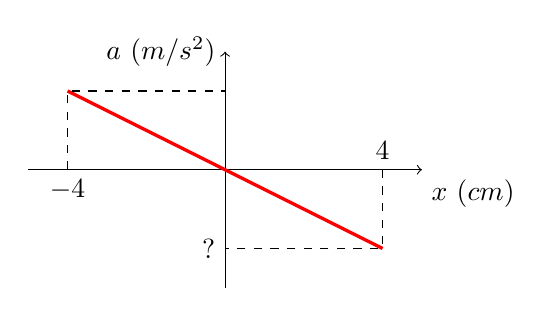
\begin{tikzpicture}
\draw[->](0,-1.5)--(0,1.5)node[left]{$a\ (m/s^2)$};
\draw[->](-2.5,0)--(2.5,0)node[below right]{$x\ (cm)$};
\draw[very thick,red](-2,1)--(2,-1);
\draw[dashed](-2,0)node[below]{$-4$}--(-2,1)--(0,1);
\draw[dashed](2,0)node[above]{$4$}--(2,-1)--(0,-1)node[left]{$?$};
\end{tikzpicture}}
\loigiai{
Ta có: $a_{\max} = \omega^2A = 400\ cm/s^2 = 4\ m/s^2$.
}
%\haidong{7}
\end{ex} \haidong{20}
%\loai{Đồ thị pha dao động}
\begin{ex}%book %[3P1-20.1K][Loai1]
\immini[thm]{Một chất điểm dao động điều hòa trên trục Ox với biên độ Ox với biên độ 10 cm. Pha dao động của vật phụ thuộc thời gian theo đồ thị như hình vẽ. Phương trình dao động của vật \textbf{gần nhất} với biểu thức nào sau đây?
\choice
{$x = 10\cos(\pi t - \dfrac{\pi}{3})$ cm}
{$x = 10\cos(\pi t + \dfrac{\pi}{3})$ cm}
{$x = 10\cos(2\pi t - \dfrac{\pi}{3})$ cm}
{\True $x = 10\cos(2\pi t + \dfrac{\pi}{3})$ cm}}{\begin{tikzpicture}[scale=1.7,thick,>=stealth',x=1cm,y=0.7cm]
\draw[->] (-3.5,0)--(1.5,0)node[above]{$t\ (s)$};
\draw[->] (0,-0.4)--(0,3.5)node[right]{$\Phi\ (rad)$};
\foreach \x in {-3.5,-3,...,1.2}
{\draw [thin,green!40!black] (\x,-0.3) --(\x,3.3);}
\foreach \y in {-0.25,0.25,...,3.3}
{\draw [dashed,thin,green!40!black] (-3.5,\y) --(1.2,\y);}
\foreach \y in {0,0.5,...,3.3}
{\draw [thin,green!40!black] (-3.5,\y) --(1.2,\y);}
\draw [red,line width = 1.5pt] (-3.7,-0.3) --(0.9,3.3);
\node at (0,0)[below right]{$O$};
\node at (1,0)[below]{$0,05$};
\node at (-1,0)[below]{$-0,05$};
\node at (-2,0)[below]{$-0,10$};
\node at (-3,0)[below]{$-0,15$};
\node at (0,0.5)[right]{$0,2$};
\node at (0,1)[right]{$0,4$};
\node at (0,1.5)[right]{$0,6$};
\node at (0,2)[right]{$0,8$};
\node at (0,2.5)[right]{$1,0$};
\node at (0,3)[right]{$1,2$};
\end{tikzpicture}
}
\loigiai{
\begin{itemize}
\item Vì pha dao động của vật là: $\Phi = \omega t + \varphi$.
\item Khi $t = -0,15\ s$ thì $\Phi = 0,1\ rad \Rightarrow 0,1 = \omega.-0,15 + \varphi$ (1)
\item Khi $t = 0,025\ s$ thì $\Phi = 1,2\ rad \Rightarrow 1,2 = \omega.0,025 + \varphi$ (2)
\item Giải (1) và (2) ta được: $\omega = \dfrac{44}{7} = 2\pi\ rad/s$ và $\varphi = \dfrac{73}{70} = \dfrac{\pi}{3}\ rad$.
\end{itemize}
}
%\haidong{3}
\end{ex} \haidong{20}
\begin{ex}%book %[3P1-20.1G][Loai1]
\immini[thm]{Một chất điểm dao động điều hòa có pha dao động của li độ quan hệ với thời gian được biểu diễn như hình vẽ. Quãng đường chất điểm đi được từ thời điểm $t_3$ đến thời điểm $t_4$ là 10 cm và $t_2 - t_1 = 0,5\ s$. Gia tốc của chất điểm tại thời điểm $t = 2018\ s$ \textbf{gần nhất} với giá trị nào sau đây?
\haicot
{17 $cm/s^2$}
{\True 22 $cm/s^2$}
{20 $cm/s^2$}
{14 $cm/s^2$}}{\begin{tikzpicture}[scale=1,thick,>=stealth']
\draw[->] (0,0)--(4.5,0)node[above]{$t\ (s)$};
\draw[->] (0,-1.3)--(0,2.5)node[right]{$\omega t+\varphi\ (rad)$};
\foreach \x in {0.5,1,...,4}
{\draw [dashed,thin,green!40!black] (\x,-1) --(\x,2);}
\foreach \y in {-1,-0.5,0.5,1,...,2}
{\draw [dashed,thin,green!40!black] (0,\y) --(4,\y);}
\node at (0,0)[left]{$O$};
\node at (0,0.5)[left]{$\dfrac{\pi}{3}$};
\draw[fill=white] (0.5,-1)circle(1pt)node[below]{$t_1$};
\draw[fill=white] (1,-1)circle(1pt)node[below]{$t_2$};
\draw[fill=white] (2,-1)circle(1pt)node[below]{$t_3$};
\draw[fill=white] (3,-1)circle(1pt)node[below]{$t_4$};
\draw[fill=white] (0,0.5)circle(1pt);
\draw[fill=white] (0,1)circle(1pt);
\draw[fill=white] (0,1.5)circle(1pt);
\draw[fill=white] (0,2)circle(1pt);
\draw[fill=white] (0,0)circle(1pt);
\draw[red,very thick](0,-1)--(3,2);
\draw[fill=white] (0,-1)circle(1pt);
\draw[fill=white] (0.5,-0.5)circle(1pt);
\draw[fill=white] (1,0)circle(1pt);
\draw[fill=white] (2,1)circle(1pt);
\draw[fill=white] (3,2)circle(1pt);
\end{tikzpicture}
}
\loigiai{
\begin{itemize}
\item Ta có $t_2 - t_1 = 0,5\ s\ \Rightarrow$ trên Ot mỗi khoảng tương ứng 0,5 s.
\item Khi $t = 0$ thì $(\omega.0 + \varphi) = - \dfrac{2\pi}{3} \Rightarrow \varphi = - \dfrac{2\pi}{3}$.
\item Khi $t = t_2 = 1\ s$ thì $(\omega.1 + \varphi) = 0 \Rightarrow \omega = \dfrac{2\pi}{3}\ rad/s \Rightarrow T = 3\ s$.
\end{itemize}
\immini{\begin{itemize}
\item Phương trình dao động có dạng $x = A\cos(\dfrac{2\pi}{3}t - \dfrac{2\pi}{3}) cm$
\item Khi $t = t_3 = 2\ s$ thì pha là $\dfrac{2\pi}{3}\ rad$.
\item Khi $t = t_4 = 3\ s$ thì pha là $\dfrac{4\pi}{3}\ rad \Rightarrow$ góc quét $\Delta\varphi = \dfrac{2\pi}{3}\ rad$ trên vòng tròn.
\item Dễ dàng tính được $S = A = 10\ cm$.
$\Rightarrow$ Phương trình dao động $x = 10\cos(\dfrac{2\pi}{3}t - \dfrac{2\pi}{3}) cm$
\item Gia tốc $a = - \left(\dfrac{2\pi}{3}\right)^2.10\cos(\dfrac{2\pi}{3}t-\dfrac{2\pi}{3})\ cm/s^2$. 
\item Khi $t = 2018 s$ thì $a = 21,9\ cm/s^2$.
\end{itemize}}{\begin{tikzpicture}[scale=1,thick,>=stealth']
\tkzInit[ymin=-3,ymax=3,xmin=-3,xmax=3]\tkzClip
\tkzDefPoints{-2.5/0/m, 2.5/0/n, 0/0/o, 0/2.5/p, 0/-2.5/q}
\tkzDefShiftPoint[o](240:2){2}
\tkzDefShiftPoint[o](120:2){1}
\tkzDefShiftPoint[o](90:2){0}
\tkzDefPointBy[projection=onto m--n](1) \tkzGetPoint{h}
\draw(o)circle(2cm);
\tkzDrawSegments[dashed](1,2)
\tkzDrawSegments(p,q)
\tkzDrawSegments[->](m,n)
\tkzDrawSegments[blue,->](o,1 o,2)
\tkzDrawPoints[size=3](o,1,h,2)
\node at (1)[above left]{$t_3$};
\node at (2)[below left]{$t_4$};
\node at (2,0)[below right]{$A$};
\node at (h)[below left]{$-\dfrac{A}{2}$};
\end{tikzpicture}
}
}
%\haidong{13}
\end{ex} \haidong{20}
\section{Con lắc lò xo}

\begin{ex}%book %[3P1Y5-1][Loai1]  
Một con lắc lò xo gồm vật nhỏ có khối lượng m và lò xo có độ cứng k, dao động điều hòa với phương trình $x=A\cos \left({\omega t+\varphi }\right)$. Mốc thế năng ở vị trí cân bằng. Cơ năng của con lắc là
\choice
{$\dfrac{1}{2}{mA}^2$}
{\True $\dfrac{1}{2}{kA}^2$}
{$\dfrac{1}{2}{mx}^2$}
{$\dfrac{1}{2}{kx}^2$}
\loigiai{
Cơ năng của con lắc là $\dfrac{1}{2}{kA}^2$. 
}
\end{ex} \haidong{20}
\begin{ex}%book %[3P1Y5-1][Loai1]  
Khi nói về cơ năng của chất điểm dao động điều hòa, phát biểu nào sau đây là \textbf{sai}? Cơ năng của chất điểm dao động điều hòa luôn luôn bằng
\choice
{thế năng ở vị trí biên}
{động năng ở vị trí cân bằng}
{\True động năng ở thời điểm ban đầu}
{tổng động năng và thế năng ở thời điểm bất kì}
\loigiai{
Cơ năng của chất điểm dao động điều hòa luôn bằng động năng ở thời điểm ban đầu là sai.
}
\end{ex} \haidong{20}
\begin{ex}%book %[3P1B5-1][Loai1] 
Nếu tăng khối lượng của con lắc lò xo lên 4 lần đồng thời giữ nguyên biên độ dao động không đổi thì cơ năng của nó
\choice
{\True không đổi}
{tăng 4 lần}
{tăng 2 lần}
{giảm $\dfrac{1}{2}$ lần}
\loigiai{
Ta có: $W=\dfrac{1}{2}kA^2$ mà k, A không đổi nên W không đổi.
}
\end{ex} \haidong{20}
\begin{ex}%book%[3P1B5-1][Loai1]%Bài 13
Phát biểu nào sau đây về động năng và thế năng trong dao động điều hoà là \textbf{không} đúng?
\choice
{Thế năng biến đổi tuần hoàn với tần số gấp 2 lần tần số của li độ}
{Động năng và thế năng biến đổi tuần hoàn cùng chu kì}
{Tổng động năng và thế năng không phụ thuộc vào thời gian}
{\True Động năng biến đổi tuần hoàn với cùng chu kì vận tốc}
\loigiai{
Trong dao động điều hòa, động năng và thế năng biến đổi tuần hoàn với chu kì bằng nửa chu kì của vận tốc.
}
\end{ex} \haidong{20}
\begin{ex}%book %[3P1B5-1][Loai1]  
Phát biểu nào sau đây về động năng và thế năng trong dao động điều hoà là \textbf{không} đúng?
\choice
{Động năng đạt giá trị cực đại khi vật chuyển động qua vị trí cân bằng}
{Động năng đạt giá trị cực tiểu khi vật ở một trong hai vị trí biên}
{Thế năng đạt giá trị cực đại khi gia tốc của vật đạt giá trị cực tiểu}
{\True Thế năng đạt giá trị cực tiểu khi gia tốc của vật đạt giá trị cực tiểu}
\loigiai{
\begin{itemize}
\item Khi vật chuyển động qua VTCB thì tốc độ của vật cực đại $\Rightarrow$ Động năng đạt giá trị cực đại nên A đúng.
\item Khi vật ở vị trí biên thì tốc độ của vật bằng 0 $\Rightarrow$ động năng của vật đạt giá trị cực tiểu nên B đúng.
\item Gia tốc của vật đạt giá trị cực tiểu tại biên dương $\Rightarrow$ thế năng đạt giá trị cực đại nên C đúng, D sai.
\end{itemize}
}
\end{ex} \haidong{20}
\begin{ex}%book
Phát biểu nào sau đây \textbf{sai}? Một con lắc lò xo nằm ngang đang thực hiện dao động điều hoà thì
\choice
{động năng của vật nặng và thế năng đàn hồi của lò xo là hai thành phần tạo thành cơ năng của con lắc}
{động năng và thế năng biến thiên tuần hoàn với cùng một tần số như nhau}
{khi vật ở một trong hai vị trí biên thì thế năng đạt giá trị cực đại}
{\True động năng và thế năng biến thiên tuần hoàn với cùng chu kì như chu kì của dao động}
\loigiai{

}
\end{ex} \haidong{20}
\begin{ex}%book
Phát biểu nào sau đây là \textbf{sai} khi nói về năng lượng của hệ dao động điều hoà?
\choice
{Hệ có thế năng cực đại khi vật ở vị trí biên dương}
{Vật có động năng cực đại khi ở vị trí cân bằng}
{Hệ có cơ năng không đổi trong suốt quá trình dao động}
{\True Hệ có thế năng bằng không khi vật ở vị trí biên âm}
\end{ex} \haidong{20}

\begin{ex}%book %[3P1Y5-1][Loai1] 
Hai con lắc lò xo dao động điều hòa cùng tần số và có biên độ lần lượt là $A_1$ , $A_2$ với $A_1<A_2$. Điều nào sau đây là đúng khi so sánh cơ năng hai con lắc?
\choice
{\True Không thể so sánh được}
{Cơ năng của con lắc thứ nhất lớn hơn}
{Cơ năng của con lắc thứ hai lớn hơn}
{Cơ năng của 2 con lắc bằng nhau}
\loigiai{
Ta có: $W=\dfrac{1}{2}kA^2$ $\Rightarrow$ không so sánh được.
}
\end{ex} \haidong{20}

\begin{ex}%book %[3P1B3-2][Loai1]  
Một con lắc lò xo gồm lò xo có độ cứng $k=200\ N/m$, vật nhỏ khối lượng m, dao động điều hòa với tần số góc $20\ rad/s$. Giá trị của m là
\choice
{100 g}
{200 g}
{400 g}
{\True 500 g}
\loigiai{
Tần số góc $\omega $ dao động của con lắc lò xo là:
$\omega =\sqrt{\dfrac{k}{m}}\Leftrightarrow 20=\sqrt{\dfrac{200}{m}}\Rightarrow m=0,5\ kg=500\ g$.
}%<MyLT1>
%\haidong{2}
\end{ex} \haidong{20}
\begin{ex}%book %[3P1-3.2B][Loai1]  
Một con lắc lò xo dao động điều hoà với biên độ $A = 8$ cm, chu kì $T = 0,5$ s. Cho biết khối lượng quả nặng là 0,4 kg. Độ cứng của lò xo bằng
\choice
{\True $k = 6,4\pi^2$ N/m}
{$k = \dfrac{0,025}{\pi^2}$ N/m}
{$k = 6400\pi^2$ N/m}
{$k = 128\pi^2$ N/m}
\loigiai{
Từ công thức: $T = 2\pi\sqrt{\dfrac{m}{k}}\Rightarrow k = \dfrac{4\pi^2m}{T^2} = 6,4\pi^2\ N/m$.
}
%\haidong{2}
\end{ex} \haidong{20}
\begin{ex}%book%[3P1-9.2K][Loai1] 
Một con lắc lò xo có khối lượng vật nhỏ là 50 g. Con lắc dao động điều hòa theo một trục cố định nằm ngang với phương trình $x = A\cos\omega t$. Cứ sau những khoảng thời gian 0,05 s thì động năng và thế năng của vật lại bằng nhau. Lấy $\pi^2 = 10$. Lò xo của con lắc có độ cứng bằng
\choice
{25 N/m}
{150 N/m}
{100 N/m}
{\True 50 N/m}
\loigiai{
\begin{itemize}
\item Ta có: $n.\dfrac{T}{4} = 0,05 \Rightarrow T = \dfrac{0,2}{n}\ s\Rightarrow \omega = \dfrac{2\pi}{T} = \dfrac{2\pi.n}{0,2} = 10n\pi\ rad/s\Rightarrow k = m\omega^2 = 0,05.(10n\pi)^2 = 50n^2$.
\item Với $n=1 \Rightarrow k=50\ N/m$.

\end{itemize}
}
%\haidong{5}
\end{ex} \haidong{20}
\begin{ex}%book%[3P1-12.1K][Loai1]
Một vật dao động điều hòa với tần số 5 Hz. Tại thời điểm $t_1$ vật có động năng bằng 3 lần thế năng. Tại thời điểm ${t_2}={t_1}+\dfrac{1}{30}$  s thì động năng của vật \textit{có thể}
\choice
{bằng $ \dfrac{1}{3} $ lần thế năng hoặc bằng cơ năng}
{bằng 3 lần thế năng hoặc bằng cơ năng}
{\True bằng 3 lần thế năng hoặc bằng không}
{bằng $ \dfrac{1}{3} $ lần thế năng hoặc bằng không}
\loigiai{
\begin{itemize}
\item $W_{\text{đ}}=3W_t\Rightarrow \left| x \right|=\dfrac{A}{2}$, không mất tính tổng quát chọn: $x=\dfrac{A}{2}$.  
\item Nếu vật qua $x=\dfrac{A}{2}\oplus,$ thì sau $ \dfrac{1}{30}=\dfrac{T}{6}$ s vật tới biên dương có $W_{\text{đ}} = 0$.  
\item Nếu vật qua $x=\dfrac{A}{2}$, thì sau $\dfrac{1}{30}=\dfrac{T}{6}$ s vật tới $x=-\dfrac{A}{2}$ có $W_{\text{đ}}=3{W_t}$.

\end{itemize}
}
%\haidong{7}
\end{ex} \haidong{20}
\begin{ex}%book %[3P1B5-2][Loai1] 
Một vật khối lượng 750 g dao động điều hoà với biên độ 4 cm; chu kì 2 s. Lấy $\pi^2 = 10$. Năng lượng dao động của vật là
\choice
{60 J}
{\True 6 mJ}
{$6.10^{-3}$ mJ}
{0,15 J}
\loigiai{
Ta có: $T=2\pi\sqrt{\dfrac{m}{k}}=2\ s \Rightarrow k=7,5\ N/m\Rightarrow W=\dfrac{1}{2}kA^2=0,006\ J$.
}
%\haidong{2}
\end{ex} \haidong{20}
\begin{ex}%book%[3P1K9-2][Loai1]
Một vật dao động điều hòa với tần số 2 Hz. Tại thời điểm $t_1$ vật có động năng bằng 3 lần thế năng. Tại thời điểm $t_2=t_1+\dfrac{1}{12}$ s thì thế năng của vật \textit{có thể} bằng
\choice
{động năng}
{0}
{\True cơ năng}
{nửa động năng}
\loigiai{
\begin{itemize}
\item $W_{\text{đ}}=3{W_t}\Rightarrow \left| x \right|=\dfrac{A}{2}$, không mất tính tổng quát chọn: $x=\dfrac{A}{2}$.  
\item Nếu vật qua $x=\dfrac{A}{2}\oplus ,$ thì sau $ \dfrac{1}{12}=\dfrac{T}{6} $ s vật tới biên dương có $W_t = W$ (cực đại).  
\item Nếu vật qua $x=\dfrac{A}{2}$, thì sau $ \dfrac{1}{12}=\dfrac{T}{6} $ s vật tới $x=-\dfrac{A}{2}$ có $W_{\text{đ}}=3{W_t}$.
\end{itemize}
}
%\haidong{5}
\end{ex} \haidong{20}
\begin{ex}%book%[3P1K9-2][Loai1]
Một con lắc lò xo gồm lò xo nhẹ và vật nhỏ khối lượng 100 g đang dao động điều hòa theo phương ngang, mốc tính thế năng tại vị trí cân bằng. Từ thời điểm $t_1 = 0$ s đến $t_2 = \dfrac{\pi}{48}\ s$, động năng của con lắc tăng từ $0,192\ J$ đến giá trị cực đại rồi giảm về $0,128\ J$. Ở thời điểm $t_2$, thế năng của con lắc bằng $0,128\ J$. Biên độ dao động của con lắc là
\choice
{7,0 cm}
{\True 11,3 cm}
{3,6 cm}
{5,7 cm}
\loigiai{
\immini{
\begin{itemize}
\item Cơ năng của con lắc là $W = W_{\text{đ}_2} + W_{t2} = 0,128 + 0,128 = 0,256$ J.
\item Xét tại thời điểm $t_2$, có $W_{\text{đ}_2} = W_{t2} \Rightarrow W_{t2} = \dfrac{W}{2} \Rightarrow x = \pm \dfrac{A}{\sqrt{2}} $. 
\item Ta biểu diễn các vị trí có li độ $ x = \pm \dfrac{A}{\sqrt{2}} $ tại các điểm $N_1,\ N_2,\ N_3,\ N_4$ như hình vẽ.
\item Tại thời điểm $t_1$, Ta có: $W_{t1} = 0,256-0,192 = 0,064\ J \Rightarrow W_{t1} = \dfrac{W}{4} \Rightarrow x = \pm \dfrac{A}{2} $.
\item Ta biểu diễn các vị trí có li độ $ x = \pm \dfrac{A}{2} $ tại các điểm $ M_1,\ M_2,\ M_3,\ M_4$ như trên hình. 
\end{itemize}
}{\begin{tikzpicture}[scale=1,thick,>=stealth']
\tkzInit[ymin=-3,ymax=3,xmin=-3,xmax=3]\tkzClip
\tkzDefPoints{-2.5/0/m, 2.5/0/n, 0/0/o, 0/2.5/p, 0/-2.5/q}
\tkzDefShiftPoint[o](-120:2){m1}
\tkzDefShiftPoint[o](-60:2){m2}
\tkzDefShiftPoint[o](60:2){m3}
\tkzDefShiftPoint[o](120:2){m4}
\tkzDefShiftPoint[o](-135:2){n1}
\tkzDefShiftPoint[o](-45:2){n2}
\tkzDefShiftPoint[o](45:2){n3}
\tkzDefShiftPoint[o](135:2){n4}
\tkzDefPointBy[projection=onto m--n](m2) \tkzGetPoint{h}
\tkzDefPointBy[projection=onto m--n](m1) \tkzGetPoint{h'}
\tkzDefPointBy[projection=onto m--n](n2) \tkzGetPoint{k}
\tkzDefPointBy[projection=onto m--n](n1) \tkzGetPoint{k'}
\draw(o)circle(2cm);
\tkzDrawSegments[dashed](m1,m4 m2,m3 n1,n4 n2,n3)
\tkzDrawSegments(p,q)
\tkzDrawSegments[->](m,n)
\tkzDrawSegments[blue,->](o,m1 o,m2 o,m4 o,m3)
\tkzDrawSegments[red,->](o,n1 o,n2 o,n4 o,n3)
\tkzDrawPoints[size=3](o,m1,h,m4,m2,m3,h',n1,k,n4,n2,n3,k')
\tkzMarkAngles[size=0.7cm,arrows=->](m1,o,n2 m3,o,n4)
\node at (m1)[below left]{$M_1$};
\node at (m2)[below right]{$M_2$};
\node at (m3)[above right]{$M_3$};
\node at (m4)[above left]{$M_4$};
\node at (n1)[below left]{$N_1$};
\node at (n2)[below right]{$N_2$};
\node at (n3)[above right]{$N_3$};
\node at (n4)[above left]{$N_4$};
\node at (2,0)[above right]{$A$};
\node at (h)[below]{$\dfrac{A}{2}$};
\node at (k')[below]{$-\dfrac{A}{\sqrt{2}}$};
\end{tikzpicture}}
\begin{itemize}
\item Mà động năng của vật có giá trị cực đại khi vật ở vị trí cân bằng nên từ thời điểm $t_1$ đến thời điểm $t_2$, vật đi từ $ M_1$ qua vị trí cân bằng theo chiều âm tới $N_2$ hoặc vật đi từ $ M_3$ qua vị trí cân bằng theo chiều dương tới $N_4$.
\item Xét cả hai trường hợp, vật cùng quay được góc $\Delta \varphi = \dfrac{\pi}{6} + \dfrac{\pi}{4} = \dfrac{5\pi}{12}$\\
$\Rightarrow \Delta t = \dfrac{5T}{24} \Rightarrow \dfrac{5T}{24} = \dfrac{\pi}{48} \Rightarrow T = \dfrac{\pi}{10} \Rightarrow \omega = 20\ rad/s$.
\item Mà $W = \dfrac{m\omega^2A^2}{2} \Rightarrow 0,256 = \dfrac{0,1.20^2A^2}{2} \Rightarrow A = 0,113\ m=11,3\ cm$.
\end{itemize}
}
%\haidong{9}
\end{ex} \haidong{20}
\begin{ex}%book%[3P1K9-2][Loai1]
Một vật dao động điều hòa với tần số là 9 Hz. Khoảng thời gian giữa hai lần liên tiếp mà thế năng bằng 3 lần động năng \textit{có thể} là
\choice
{28 ms}
{\True 37 ms}
{56 ms}
{9 ms}
\loigiai{
\immini{
\begin{itemize}
\item Ta có: $W_t = 3W_\text{đ} \Rightarrow W_t = \dfrac{3W}{4} \Rightarrow x = \pm \dfrac{A\sqrt{3}}{2}$. 
\item Ta biểu diễn vị trí có thế năng bằng 3 lần động năng tại các điểm $ M_1,\ M_2,\ M_3,\ M_4$ như hình vẽ.
\item Ta xét trường hợp 1: vật đi từ $ M_1$ đến $ M_2$ hoặc vật đi từ $ M_3$ đến $ M_4$ thì
$\Delta \varphi_1 = \dfrac{\pi}{3} + \dfrac{\pi}{3} = \dfrac{2\pi}{3} \Rightarrow \Delta t_1 = \dfrac{T}{3} = \dfrac{1}{3f} = \dfrac{1}{27}s = 37\ ms$.
\item Ta xét trường hợp 2: vật đi từ $ M_2$ đến $ M_3$ và trường hợp vật đi từ $ M_4$ đến $ M_1$ thì
$\Delta \varphi_2 = \dfrac{\pi}{6} + \dfrac{\pi}{6} = \dfrac{\pi}{3} \Rightarrow \Delta t_2 = \dfrac{T}{6} = \dfrac{1}{6f} = \dfrac{1}{54} \ s = 18,5\ ms$.
\end{itemize}
}{\begin{tikzpicture}[scale=1,thick,>=stealth']
\tkzInit[ymin=-3,ymax=3,xmin=-3,xmax=3]\tkzClip
\tkzDefPoints{-2.5/0/m, 2.5/0/n, 0/0/o, 0/2.5/p, 0/-2.5/q}
\tkzDefShiftPoint[o](-150:2){1}
\tkzDefShiftPoint[o](-30:2){2}
\tkzDefShiftPoint[o](30:2){3}
\tkzDefShiftPoint[o](150:2){4}
\tkzDefPointBy[projection=onto m--n](2) \tkzGetPoint{h}
\tkzDefPointBy[projection=onto m--n](1) \tkzGetPoint{h'}
\draw(o)circle(2cm);
\tkzDrawSegments[dashed](1,4 2,3)
\tkzDrawSegments(p,q)
\tkzDrawSegments[->](m,n)
\tkzDrawSegments[blue,->](o,1 o,2 o,4 o,3)
\tkzDrawPoints[size=3](o,1,h,4,2,3,h')
\tkzMarkAngles[size=0.7cm,arrows=->](1,o,2)
\tkzLabelAngle[pos=1](1,o,q){$\Delta \varphi_1$}
\tkzMarkAngles[size=0.5cm,arrows=->](2,o,3)
\tkzLabelAngle[pos=0.9](n,o,3){$\Delta \varphi_2$}
\node at (1)[below left]{$M_1$};
\node at (2)[below right]{$M_2$};
\node at (3)[above right]{$M_3$};
\node at (4)[above left]{$M_4$};
\node at (2,0)[above right]{$A$};
\node at (h')[below]{$-\dfrac{A\sqrt{3}}{2}$};
\node at (h)[below]{$\dfrac{A\sqrt{3}}{2}$};
\end{tikzpicture}}
}
%\haidong{5}
\end{ex} \haidong{20}
\begin{ex}%book %[3P1B5-2][Loai1] 
Một vật nhỏ có khối lượng bằng 50 g, dao động điều hòa với tần số góc bằng 6 rad/s. Động năng cực đại của vật là $3,6.10^{-4}$ J. Biên độ dao động của vật là 
\choice
{4 cm}
{\True 2 cm}
{3 cm}
{7 cm}
\loigiai{
Ta có: $W_{\text{đ}\max} = W = \dfrac{m\omega^2A^2}{2} \Rightarrow A = \sqrt{\dfrac{2W_{\text{đmax}}}{m\omega^2}} = \sqrt{\dfrac{2.3,6.10^{-4}}{0,05.6^2}} = 0,02\ m=2\ cm$.
}
%\haidong{2}
\end{ex} \haidong{20}
\begin{ex}%book %[3P1B5-3][Loai1]   
\nguon{CĐ - 2010} Một vật dao động điều hòa với biên độ 6 cm. Mốc thế năng ở vị trí cân bằng. Khi vật có động năng bằng $\dfrac{3}{4}$ lần cơ năng thì vật cách vị trí cân bằng một đoạn
\choice
{6 cm}
{4,5 cm}
{4 cm}
{\True 3 cm}
\loigiai{Vật cách vị trí cân bằng một đoạn
\begin{align*}
W_{\text{đ}}=\dfrac{3}{4}{W}\Rightarrow W_t=\dfrac{1}{4}{W}\Rightarrow \dfrac{kx^2}{2}=\dfrac{1}{4}\dfrac{kA^2}{2}\Rightarrow x=\pm \dfrac{A}{2}=\pm 3\ cm.
\end{align*}}
%\haidong{3}
\end{ex} \haidong{20}
\begin{ex}%book%[3P1K5-3][Loai1]
Một vật dao động điều hòa trên trục Ox. Mối liên hệ giữa li độ x, tốc độ v và tần số góc $ \omega $ của vật dao động khi thế năng bằng 3 lần động năng của hệ là
\choice
{$ \omega =2\left| x \right|v$}
{$ 3v=2\omega \left| x \right|$}
{$ \left| x \right|=2\omega v$}
{\True $ \omega \left| x \right|=v\sqrt{3}$}
\loigiai{
\begin{itemize}
\item Ta có: $W_t=3W_{\text{đ}}\Rightarrow W_{\text{đ}}=\dfrac{1}{3}W_t\Rightarrow \left| x \right|=\dfrac{A\sqrt{3}}{2}\Rightarrow v=\dfrac{\omega A}{2}\Rightarrow \omega \left| x \right|=v\sqrt{3}$.
\item 
\end{itemize}
}
%\haidong{7}
\end{ex} \haidong{20}
\begin{ex}%book %[3P1B5-3][Loai1] 
Một vật nhỏ khối lượng 100 g đang dao động điều hòa với chu kì là 0,2 s. Lấy $\pi^2 = 10$, mốc thế năng tại vị trí cân bằng. Tại li độ $3\sqrt{2}$ cm, tỉ số động năng và thế năng bằng 1. Cơ năng toàn phần của dao động là
\choice
{1 J}
{0,12 J}
{\True 0,18 J}
{0,2 J}
\loigiai{
\begin{itemize}
\item Ta có: $\omega = \dfrac{2\pi}{T} = 10\pi \ rad/s\Rightarrow W_t = \dfrac{m\omega^2x^2}{2} = \dfrac{0,1.(10\pi)^2.(0,03\sqrt{2})^2}{2} = 0,09\ J$.
\item $\dfrac{W_{\text{đ}}}{W_t} = \dfrac{W_{\text{đ}}}{0,09} = 1 \Rightarrow W_d = 0,09\ J\Rightarrow W = W_d + W_t = 0,09 + 0,09 = 0,18\ J$.
\end{itemize}
}
%\haidong{6}
\end{ex} \haidong{20}
\begin{ex}%book %[3P1K5-1][Loai1] 
Trong dao động điều hòa của con lắc lò xo thì đồ thị của thế năng theo li độ có dạng
\choice
{Đường thẳng}
{elip}
{Hình $\sin$}
{\True parabol}
\loigiai{
Ta có: $W_t = \dfrac{1}{2}kx^2 \Rightarrow$ Đồ thị của thế năng theo li độ có dạng parabol.
}
%\haidong{5}
\end{ex} \haidong{20}
\begin{ex}%book%[3P1K9-2][Loai1] 
Một vật dao động điều hòa dọc theo trục tọa độ nằm ngang Ox với chu kì T, vị trí cân bằng và mốc thế năng ở gốc tọa độ. Tính từ lúc vật có li độ dương lớn nhất, thời điểm đầu tiên mà động năng và thế năng của vật bằng nhau là
\choice
{\True $\dfrac{T}{8}$}
{$\dfrac{T}{6}$}
{$\dfrac{T}{12}$}
{$\dfrac{T}{4}$}
\loigiai{
\immini{\begin{itemize}
\item Ta có: $W_{\text{đ}} = W_t \Rightarrow W_t = \dfrac{W}{2} \Rightarrow x = \pm \dfrac{A}{\sqrt{2}}$. 
\item Ta biểu diễn vị trí ban đầu và vị trí có li độ $x = \pm \dfrac{A}{\sqrt{2}}$ tại các điểm $ M,\ N_1,\ N_2,\ N_3,\ N_4$ như hình vẽ.
\item Từ lúc vật có li độ dương lớn nhất, thời điểm đầu tiên mà động năng và thế năng của vật bằng nhau ứng với thời gian để để vật đi từ M đến $N_1$ trên đường tròn
$\Rightarrow \Delta \varphi = \dfrac{\pi}{4} \Rightarrow \Delta t = \dfrac{T}{8}$.
\end{itemize}}{\begin{tikzpicture}[scale=1,thick,>=stealth']
\tkzInit[ymin=-3,ymax=3,xmin=-3,xmax=3]\tkzClip
\tkzDefPoints{-2.5/0/m, 2.5/0/n, 0/0/o, 0/2.5/p, 0/-2.5/q}
\tkzDefShiftPoint[o](0:2){0}
\tkzDefShiftPoint[o](-135:2){1}
\tkzDefShiftPoint[o](-45:2){2}
\tkzDefShiftPoint[o](45:2){3}
\tkzDefShiftPoint[o](135:2){4}
\tkzDefPointBy[projection=onto m--n](2) \tkzGetPoint{h}
\tkzDefPointBy[projection=onto m--n](1) \tkzGetPoint{h'}
\draw(o)circle(2cm);
\tkzDrawSegments[dashed](1,4 2,3)
\tkzDrawSegments(p,q)
\tkzDrawSegments[->](m,n)
\tkzDrawSegments[blue,->](o,1 o,2 o,4 o,3 o,0)
\tkzDrawPoints[size=3](o,1,h,4,2,3,h')
\tkzMarkAngles[size=0.5cm,arrows=->](0,o,3)
\node at (0)[above right]{$M$};
\node at (1)[below left]{$N_3$};
\node at (2)[below right]{$N_4$};
\node at (3)[above right]{$N_1$};
\node at (4)[above left]{$N_2$};
\node at (2,0)[below right]{$A$};
\node at (h')[below]{$-A\sqrt{2}$};
\node at (h)[below]{$A\sqrt{2}$};
\end{tikzpicture}}
}
%\haidong{4}
\end{ex} \haidong{20}
\begin{ex}%book%[3P1G9-2][Loai1]  
Một vật dao động điều hòa với phương trình $x=6\cos\left(10\pi t+\dfrac{2\pi }{3} \right)$ cm. Thời điểm thứ 100 vật có động năng bằng thế năng và đang chuyển động về phía vị trí cân bằng là
\choice
{19,92 s}
{\True 9,96 s}
{20,12 s}
{10,06 s}
\loigiai{
\begin{itemize}
\item Chu kì: $T=\dfrac{2\pi }{\omega }=0,2\ s$. 
\item Trong một chu kì chỉ có hai thời điểm động năng bằng thế năng và vật đang chuyển động về phía vị trí cân bằng. 
\item Hai thời điểm đầu tiên là $t_1$ và $t_2$. 
\item Để tìm các thời điểm tiếp theo ta làm như sau: 
$\dfrac{\text{Số lần }}{2}=n\left\{ \begin{aligned}
& \text{dư}\ 1: t=nT+t_1 \\
& \text{dư}\ 2: t=nT+t_2 \\ 
\end{aligned} \right.$ 
\item Ta nhận thấy: $\dfrac{100}{2}=49$ dư 2 $\Rightarrow t=49T+t_2$ nên ta chỉ cần tìm $t_2$:\\
$t_2=\dfrac{T}{6}+\dfrac{T}{2}+\dfrac{T}{8}=\dfrac{19T}{24}\Rightarrow t_{100}=49T+\dfrac{19T}{24}\approx 9,96\ s$.
\end{itemize}}
%\haidong{7}
\end{ex} \haidong{20}
\begin{ex}%book%[3P1K9-2][Loai1]  
Một con lắc lò xo đang dao động điều hòa với phương trình $x = A\cos\omega t$. Người ta thấy cứ sau $0,5\ s$ động năng lại bằng thế năng thì tần số góc dao động của con lắc sẽ là
\choice
{\True $\pi\ rad/s$}
{$0,5\pi\ rad/s$}
{$4\pi\ rad/s$}
{$2\pi\ rad/s$}
\loigiai{
\begin{itemize}
\item Trong dao động điều hòa, cứ $\dfrac{T}{4}$ thì động năng lại bằng thế năng.
\item Theo đó ta có: $0,5=\dfrac{T}{4}\Rightarrow T = 2\ s \Rightarrow \omega = \pi \ rad/s$.
\end{itemize}
}
%\haidong{6}
\end{ex} \haidong{20}
\begin{ex}%book
Một chất điểm dao động điều hoà. Biết khoảng thời gian giữa 5 lần liên tiếp động năng của chất điểm bằng thế năng của nó là 0,4 s. Tần số của dao động là
\choice
{\True 2,5 Hz}
{3,125 Hz}
{5 Hz}
{6,25 Hz}
\loigiai{
\begin{itemize}
\item $T=0,4\ s\Rightarrow f=2,5\ Hz$.

\end{itemize}
}
%\haidong{7}
\end{ex} \haidong{20}
\begin{ex}%book%[3P1K9-2][Loai1]
Một chất điểm dao động điều hòa với chu kì T và có năng lượng dao động W. Gọi $W_{\text{đ}}$ là động năng tức thời của chất điểm. Trong một chu kì khoảng thời gian mà $W_{\text{đ}} \geq 0,25W$ là
\choice
{\True $ \dfrac{2T}{3}$}
{$ \dfrac{T}{2}$}
{$ \dfrac{T}{6}$}
{$ \dfrac{T}{3}$}
\loigiai{
\begin{itemize}
\item $W_{\text{đ}} = 0,25W \Leftrightarrow  x=\pm \dfrac{A\sqrt{3}}{2}.$ 
\item Trong một chu kì:
\begin{center}
\begin{tikzpicture}
\tkzDefPoints{0/0/o, 5/0/a, 4.325/0/b, 3.525/0/c, 2.5/0/d,  -5/0/h, -4.325/0/g, -3.525/0/f, -2.5/0/e, -6/0/x', 6/0/x}
\tkzDefShiftPoint[o](-90:0.5cm){o1}
\tkzDefShiftPoint[o](-90:1.2cm){o2}
\tkzDefShiftPoint[g](-90:0.5cm){g1}
\tkzDefShiftPoint[b](-90:0.5cm){b1}
\tkzDefShiftPoint[a](-90:0.5cm){a1}
\tkzDefShiftPoint[a](-90:1.2cm){a2}
\tkzDefShiftPoint[b](-90:1.2cm){b2}
\tkzDefShiftPoint[g](-90:1.2cm){g2}
\tkzDefShiftPoint[h](-90:1.2cm){h2}
\tkzDefShiftPoint[h](-90:0.5cm){h1}
\tkzDrawSegments[blue,->,very thick](x',x)
\tkzDrawPoints[size=5,fill=black](o,a,b,c,d,e,f,g,h)
\tkzLabelPoint[above](o){\tiny $O$}
\tkzLabelPoint[above](a){\tiny$A$}
\tkzLabelPoint[above](b){\tiny$\dfrac{A\sqrt{3}}{2}$}
\tkzLabelPoint[above](c){\tiny$\dfrac{A\sqrt{2}}{2}$}
\tkzLabelPoint[above](d){\tiny$\dfrac{A}{2}$}
\tkzLabelPoint[above](h){\tiny$-A$}
\tkzLabelPoint[above](g){\tiny $-\dfrac{A\sqrt{3}}{2}$}
\tkzLabelPoint[above](f){\tiny$-\dfrac{A\sqrt{2}}{2}$}
\tkzLabelPoint[above](e){\tiny$-\dfrac{A}{2}$}
\tkzLabelPoint[above](x){\tiny$x$}
\tkzDrawSegments[very thick,red](b1,g1 b2,g2)
\tkzDrawSegments[dashed,very thick,red](a1,a2 b1,a1 g2,h2 h2,h1 g1,h1 a2,b2)
\end{tikzpicture}
\end{center}
\item $W_{\text{đ}} \geq 0,25W$ khi gần vị trí cân bằng (nét liền) $\Rightarrow  \Delta t=\dfrac{2T}{3}$.

\end{itemize}
}
%\haidong{6}
\end{ex} \haidong{20}
\begin{ex}%book %[3P1-6.2B][Loai1] 
\nguon{QG - 2018} Một con lắc lò xo dao động điều hòa theo phương ngang với biên độ 3 cm. Trong quá trình dao động chiều dài lớn nhất của lò xo là 25 cm. Khi vật nhỏ của con lắc đi qua vị trí cân bằng thì chiều dài của lò xo là
\choice
{19 cm}
{18 cm}
{31 cm}
{\True 22 cm}
\loigiai{
Chiều dài lò xo ở vị trí cân bằng: $\ell_{cb}=\ell_{\max}-A=22\ cm$.
}
%\haidong{6}
\end{ex} \haidong{20}
\begin{ex}%book%[3P1-10.1K][Loai1]
Một con lắc lò xo treo thẳng đứng có vật nhỏ dao động điều hòa với phương trình $x = 5\cos (20t + \pi )$ cm. Lấy $g = 10\ m/s^2$. Trục Ox thẳng đứng hướng lên. Kể từ $t = 0$, thời điểm vật qua vị trí lò xo không biến dạng lần đầu tiên là
\choice
{\True $ \dfrac{\pi}{30} $ s}
{$ \dfrac{\pi}{15} $ s}
{$ \dfrac{\pi}{10} $ s}
{$ \dfrac{\pi}{5} $ s}
\loigiai{
\begin{itemize}
\item $ \Delta \ell_0  = 2,5\ cm =  \dfrac{A}{2} $.
\item Tại $t = 0$: $x = -A$, Ox hướng lên $\Rightarrow$ vật ở biên dưới.
\item Thời gian ngắn nhất đi từ biên dưới tới vị trí lò xo không biến dạng là: $ \Delta t=\dfrac{T}{3}=\dfrac{\pi}{30} $ s.

\end{itemize}
}
%\haidong{10}
\end{ex} \haidong{20}
\begin{ex}%book%[3P1-10.2K][Loai1]
Con lắc lò xo treo thẳng đứng dao động điều hòa với chu kì T. Tại vị trí cân bằng lò xo dãn $\Delta \ell_0$. Khoảng thời gian lò xo bị nén trong một chu kì là 0,25T. Biên độ dao động của vật là
\choice
{$\dfrac{3}{\sqrt{2}}\Delta \ell_0 $}
{\True $\sqrt{2}\Delta \ell_0 $}
{$2\Delta \ell_0 $}
{$1,5\Delta \ell_0 $}
\loigiai{
Trong một chu kì thời gian nén là $ \dfrac{T}{4}  \Rightarrow$ vật đi từ biên trên về vị trí lò xo không biến dạng là $ \dfrac{T}{8}  \Rightarrow \Delta \ell_0 =   \dfrac{A\sqrt{2}}{2} \Rightarrow A=\sqrt{2}\Delta \ell_0$}
%\haidong{5}
\end{ex} \haidong{20}
\begin{ex}%book
Một con lắc lò xo dao động điều hòa nằm ngang với lò xo có độ cứng $k$, vật nặng có khối lượng $m$.
\choiceTF[t]
{\True Vị trí cân bằng của dao động cũng là vị trí lò xo có chiều dài tự nhiên}
{\True Chu kì dao động là $T=2 \pi \sqrt{\dfrac{m}{k}}$}
{Tần số dao động là $f=\dfrac{1}{2 \pi} \sqrt{\dfrac{m}{k}}$}
{\True Khoảng thời gian ngắn nhất vật đi từ biên về vị trí cân bằng là $t=\dfrac{T}{4}$}
\loigiai{
\begin{itemchoice}
\itemch 
\itemch 
\itemch  Tần số dao động là $f=\dfrac{1}{2 \pi} \sqrt{\dfrac{k}{m}}$.
\itemch 
\end{itemchoice}
}
%\haidong{3}
\end{ex} \haidong{20}
\begin{ex}%book
Một con lắc lò xo dao động trên mặt phẳng nằm ngang với phương trình $x=5 \cos \left(5 \pi t-\dfrac{\pi}{4}\right)\ cm$. Khi vật ở vị trí cân bằng lò xo có chiều dài là $30 \ cm$.
\choiceTF[t]
{Biên độ dao động vật là $5 \pi\ cm$}
{Tại vị trí $t=0$ vật có li độ $x=5 \sqrt{2}\ cm$}
{\True Tốc độ cực đại trong quá trình dao động là $v=25 \pi\ cm/s$}
{\True Chiều dài cực đại lò xo trong quá trình dao động là $35 \ cm$}
\loigiai{
\begin{itemchoice}
\itemch Biên độ dao động vật là $5\ cm$.
\itemch Tại vị trí $t=0$ vật có li độ $x= \dfrac{5\sqrt{2}}{2}\ cm$.
\itemch
\itemch
\end{itemchoice}
}
%\haidong{3}
\end{ex} \haidong{20}
\begin{ex}%book
Một vật có khối lượng $m=100 \ g$ được gắn vào lo xo có độ cứng $k=100 \ N/m$. Kích thích cho con lắc dao động điều hòa theo phương ngang. Trong quá trình dao động, sự biến thiên chiều dài lớn nhất của lò xo là $5 \ cm$.
\choiceTF[t]
{Khi vật đi đến biên thì vận tốc vật lớn nhất}
{Tần số góc dao động là $5 \ Hz$}
{Thời gian ngắn nhất giữa hai lần tốc độ cực đại là một chu kì}
{\True Độ lớn gia tốc cực đại trong quá trình dao động là $50 \ m/s^2$}
\loigiai{
\begin{itemchoice}
\itemch Khi vật đi đến biên thì vận tốc vật bằng không.
\itemch Tần số góc dao động là $\omega=\sqrt{\dfrac{k}{m}}=\sqrt{\dfrac{100}{0,1}}=10 \sqrt{10} rad/s$.
\itemch Thời gian ngắn nhất giữa hai lần tốc độ cực đại là $1 / 2$ chu kì.
\itemch
\end{itemchoice}
}
%\haidong{3}
\end{ex} \haidong{20}
\begin{ex}%book
Một vật có khối lượng $m=50 \ g$ được gắn vào lo xo có độ cứng $k=20 \ N/m$. Kích thích cho vật dao động điều hòa bằng cách truyền cho vật vận tốc $v=1 \ m/s$ ở vị trí cân bằng theo chiều âm.
\choiceTF[t]
{\True Ở thời điểm $t=0$ vật ở vị trí lò xo có chiều dài tự nhiên}
{Tần số góc dao động là $\omega=200\ rad/s$}
{Phương trình dao động của vật là $x=5 \cos (20 t-\dfrac{\pi}{2})\ cm$}
{\True Khoảng thời gian giữa hai lần vận tốc vật đạt cực đại có thể là $t=\pi\ s$}
\loigiai{
\begin{itemchoice}
\itemch
\itemch Tần số góc dao động là $\omega=\sqrt{\dfrac{k}{m}}=20\ rad/s$.
\itemch Phương trình dao động của vật là $x=5 \cos (20 t+\pi / 2)\ cm$.
\itemch Khoảng thời gian giữa hai lần vận tốc vật đạt cực đại có thể là $t=k \dfrac{T}{2}=k . \dfrac{\pi}{10} khi k=10 \Rightarrow t=\pi\ s$.
\end{itemchoice}
}
%\haidong{4}
\end{ex} \haidong{20}
\begin{ex}%book
Một lò xo có độ cứng $k=100 \ N/m$ được gắn với vật có khối lượng $m$. Kích thích để vật dao động điều hòa trên phương mặt phẳng ngang với biên độ $10 \ cm$.
\choiceTF[t]
{\True Trong quá trình dao động, thời gian lò xo nén bằng thời gian lò xo dãn}
{\True Độ dãn cực đại của lò trong quá trình dao động là $0,1 \ m$}
{Nếu chu kì lò xo là $2 \ s$ thì khối lượng vật là $1 \ kg$}
{Vận tốc cực tiểu trong quá trình dao động là 0}
\loigiai{
\begin{itemchoice}
\itemch 
\itemch
\itemch Nếu chu kì lò xo là $2 \ s$ thì khối lượng vật là $T=2 \pi \sqrt{\dfrac{m}{k}} \Rightarrow m=10 \ kg$.
\itemch Vận tốc cực tiểu trong quá trình dao động là $-\omega\ A$.
\end{itemchoice}
}
%\haidong{4}
\end{ex} \haidong{20}
\begin{ex}%book
Một lò xo treo thẳng đứng có độ cứng $k=100 \ N/m$ được gắn với vật có khối lượng $m=1 \ kg$. Trong quá trình dao động chiều dài lò xo biến thiên từ $28 \ cm$ đến $36 \ cm$. Lấy $g=10 \ m/s^2$.
\choiceTF[t]
{\True Biên độ dao động là $4 \ cm$}
{Chu kì dao động con lắc lò xo là $T=2\ s$}
{\True Vận tốc cực tiểu trong quá trình dao động là $-0,4 \ m/s$}
{Trong một chu kì dao động, thời gian lò xo nén lớn hơn thời gian lò xo dãn}
\loigiai{
\begin{itemchoice}
\itemch Biên độ dao động là $A=\dfrac{\ell_{\max}-\ell_{\min}}{2}=4 \ cm$.
\itemch Chu kì dao động con lắc lò xo là $T=2 \pi \sqrt{\dfrac{m}{k}}=\dfrac{\pi}{5}\ s$.
\itemch Vận tốc cực tiểu trong quá trình dao động là $v_{\text {min}}=-\omega A=-\dfrac{2 \pi}{\pi / 5} . 0,04=-0,4 \ m/s$.
\itemch $\Delta \ell_0=\dfrac{g}{\omega^2}=0,1 \ m \Rightarrow A<\Delta \ell_0$ nên lò xo luôn dãn.
\end{itemchoice}
}
%\haidong{5}
\end{ex} \haidong{20}
\begin{ex}%book%[3P1KA-2][Loai1]
Con lắc lò xo treo thẳng đứng gồm lò xo và vật nhỏ. Khi vật nhỏ nằm cân bằng lò xo dãn 3 cm. Kích thích cho cho lắc dao động với biên độ $3\sqrt{2}$ cm. Tỉ số thời gian lò xo bị nén so với thời gian bị dãn trong một chu kì là
\choice
{3}
{\True $\dfrac{1}{3}$}
{2}
{$\dfrac{1}{2}$}
\loigiai{
\begin{itemize}
\item $\Delta \ell =\dfrac{A\sqrt{2}}{2} \Rightarrow$ Trong một chu kì, khoảng thời gian lò xo nén là $\dfrac{T}{4}$, dãn là $\dfrac{3T}{4}$.

\end{itemize}
}
%\haidong{7}
\end{ex} \haidong{20}
\begin{ex}%book%[3P1KA-1][Loai1]
Một con lắc lò xo treo vào một điểm cố định, dao động điều hòa theo phương thẳng đứng với chu kì T. Trong quá trình dao động, lực đàn hồi lớn nhất là 9 N, lực đàn hồi ở vị trí cân bằng là 3 N. Khoảng thời gian từ lúc độ lớn lực đàn hồi lớn nhất đến khi độ lớn lực đàn hồi nhỏ nhất là
\choice
{$ \dfrac{T}{6}$}
{$ \dfrac{T}{4}$}
{\True $ \dfrac{T}{3}$}
{$ \dfrac{T}{2}$}
\loigiai{
\begin{itemize}
\item Ta có: $\left|F_\text{đh}\right|_{\max}=k\left( \Delta \ell_0 +A \right)=9\ N$ và $\left|F_\text{đh}\right|_0=k\Delta \ell_0 =3\ N \Rightarrow  \Delta \ell_0 =\dfrac{A}{2} \Rightarrow \Delta t=\dfrac{T}{3}$.

\end{itemize}

}
%\haidong{7}
\end{ex} \haidong{20}
\begin{ex}%book%[3P1K6-2][Loai1] 
Con lắc lò xo treo thẳng đứng với đầu cố định của lò xo ở trên cao, quả nặng ở dưới thấp. Con lắc đang dao động điều hòa trên phương thẳng đứng, quanh vị trí cân bằng, với tần số bằng $\pi$ Hz. Biết tốc độ cực đại của lò xo trong quá trình dao động là 1 m/s. Cho gia tốc trọng trường $g = \pi^2 = 10\ m/s^2$. Độ nén cực đại của lò xo là
\choice
{10 cm}
{\True 2,5 cm}
{5 cm}
{2 cm}
\loigiai{
\begin{itemize}
\item Ta có: $\omega = 2\pi.f = 2\pi.\pi = 20\ rad/s$.
\item Tại vị trí cân bằng, lò xo dãn một đoạn $\Delta \ell_0 = \dfrac{g}{\omega^2} = \dfrac{10}{20^2} = 0,025\ m = 2,5\ cm$.
\item Mà $A = \dfrac{v_{\max}}{\omega} = \dfrac{1}{20} = 0,05\ m = 5\ cm$.
\item Độ nén lớn nhất của lò xo trong quá trình dao động là $\ell = A- \Delta \ell_0 = 5-2,5 = 2,5\ cm$.
\end{itemize}
}
%\haidong{8}
\end{ex} \haidong{20}
\begin{ex}%book%[3P1K6-2][Loai1]%Bài 15 dạng 1
Một con lắc lò xo treo thẳng đứng tại nơi có $g = 10\ m/s^2$. Vật đang cân bằng thì lò xo dãn 5 cm. Kéo vật xuống dưới vị trí cân bằng 1 cm rồi truyền cho nó tốc độ $v_0$. Sau đó vật dao động điều hòa với tốc độ cực đại $30\sqrt{2}$ cm/s. Giá trị của $v_0$ là
\choice
{\True 40 cm/s}
{30 cm/s}
{20 cm/s}
{15 cm/s}
\loigiai{
\begin{itemize}
\item Ta có: $\Delta \ell_0 = 5\ cm \Rightarrow \omega  = 10\sqrt{2}\  rad/s,\ v_{\max} =  30\sqrt{2}\ cm/s \Rightarrow A = 3\ cm$.
\item Khi truyền tốc độ $v_0$, vật đang có $\left|x\right| = 1\ cm \Rightarrow v_0=\omega \sqrt{A^2-x^2}=  40\ cm/s.$
\end{itemize}
}
%\haidong{12}
\end{ex} \haidong{20}
\begin{ex}%book%[3P1K7-2][Loai1]  
Một con lắc lò xo gồm vật nặng khối lượng $m=0,1\ kg$ và lò xo có độ cứng $k=40\ N/m$ treo thẳng đứng. Cho con lắc dao động với biên độ 3 cm. Lấy $g=10\ m/s^2.$ Lực cực đại mà lò xo tác dụng vào điểm treo là
\choice
{$0,2\ N$}
{$0,1\ N$}
{\True $2,2\ N$}
{$1\ N$}
\loigiai{
\begin{itemize}
\item Tại vị trí cân bằng, lò xo đã dãn một đoạn $\Delta \ell_0$. Vật nặng chịu tác dụng của hai lực cân bằng, trọng lực và lực đàn hồi.
\item Vậy:
$P=F_0\Leftrightarrow m.g=k.\left|{\Delta \ell_0}\right|\Rightarrow \Delta \ell_0=\dfrac{m.g}{k}=\dfrac{{0,1.10}}{{40}}=0,025m=2,5\ cm$
\item Lực đàn hồi cực đại tác dụng lên vật là:
$F_{dh\max }=k.(\Delta \ell_0+A)=40.(0,025+0,03)=2,2\ N$
\end{itemize}
}
%\haidong{4}
\end{ex} \haidong{20}
\begin{ex}%book%[3P1K7-2][Loai1]
Một con lắc lò xo thẳng đứng dao động điều hòa theo phương Ox chiều dương hướng từ trên xuống. Độ cứng lò xo là 40 N/m. Khi qua li độ $x = 1,5$ cm vật chịu lực kéo đàn hồi của lò xo có độ lớn 1,6 N. Lấy $g = 10\ m/s^2$. Khối lượng vật nặng của con lắc là
\choice
{\True 100 g}
{120 g }
{50 g}
{150 g}
\loigiai{
\begin{itemize}
\item Khi vật có $x = 1,5$ cm, Ox hướng xuống $\Rightarrow$ vật đang ở dưới vị trí cân bằng O đoạn 1,5cm
\item $\Rightarrow$ Lò xo đang dãn: $\Delta \ell + 0,015$ m $\Rightarrow$ $\left|F\right| = k(\Delta \ell + 0,015) = 1,6$ N $\Rightarrow$ $\Delta \ell = 0,025$ m $\Rightarrow$ $\omega  = 20$ rad/s $\Rightarrow$ $m = 0,1$ kg.
\end{itemize}
}%<MyLT1>
%\haidong{7}
\end{ex} \haidong{20}
\begin{ex}%book%[3P1G7-2][Loai1] 

Một con lắc lò xo treo thẳng đứng tại một nơi có gia tốc rơi tự do $g=10\ m/s^2$, có độ cứng của lò xo $k = 50$ N/m. Khi vật dao động thì lực kéo cực đại và lực nén cực đại của lò xo lên giá treo lần lượt là 4 N và 2 N. Vận tốc cực đại của vật là
\choice
{$30\sqrt2$ cm/s}
{$40\sqrt5$ cm/s}
{\True $60\sqrt5$ cm/s}
{$50\sqrt5$ cm/s}
\loigiai{
\begin{itemize}
\item Ta có: $F_{kmax} = 50\left(\Delta \ell_0 + A\right) = 4$ (1); 
$F_{nmax} = 50\left(A - \Delta \ell_0 \right) = 2$ (2)
\item Từ (1) và (2) $\Rightarrow A = 0,06\ m$; $\Delta \ell_0 = 0,02\ m$
\item $v_{max} = A.\omega = A.\sqrt{\dfrac{g}{\Delta \ell_0}} = 0,06.\sqrt{\dfrac{10}{0,02}} = \dfrac{3\sqrt{5}}{5}m/s = 60\sqrt{5} cm/s$
\end{itemize}
}
%\haidong{7}
\end{ex} \haidong{20}
\begin{ex}%book%[3P1K7-2][Loai1]
Một con lắc lò xo dao động điều hoà theo phương thẳng đứng. Thời gian quả cầu đi từ vị trí cao nhất tới vị trí thấp nhất là 0,2 s; tỉ số giữa độ lớn lực đàn hồi lò xo và trọng lực vật nặng khi nó ở vị trí thấp nhất là $\dfrac{7}{4}$. Biên độ dao động của con lắc là
\choice
{2 cm}
{\True 3 cm}
{4 cm}
{5 cm}
\loigiai{
\begin{itemize}
\item T = 0,2s $\Rightarrow$ T = 0,4s $\Rightarrow$ $\Delta \ell = 4$ cm.
\item Ở vị trí thấp nhất: $\dfrac{{{\left| F \right|}_{h}}}{P}=\dfrac{k\left( \Delta \ell+A \right)}{mg}=\dfrac{7}{4}\Rightarrow \dfrac{\Delta \ell+A}{\Delta \ell}=\dfrac{7}{4}\Rightarrow $A = 3cm.
\end{itemize}
}
%\haidong{5}
\end{ex} \haidong{20}
\begin{ex}%book%[3P1-6.2K][Loai1]
Cho một con lắc lò xo được treo trên phương thẳng đứng. Biết rằng khi vật nhỏ ở vị trí cân bằng thì lò xo giãn 2,5 cm, và gia tốc trọng trường bằng $10\ m/s^2$. Chọn trục Ox hướng thẳng đứng xuống dưới, gốc O trùng vị trí cân bằng. Đưa vật theo phương thẳng đứng tới vị trí lò xo giãn 10,5 cm rồi buông nhẹ. Chọn thời điểm ban đầu $t = 0$ lúc vật đi qua vị trí có li độ 4 cm theo chiều dương lần đầu tiên. Phương trình dao động của vật nhỏ là
\choice
{$x=7\cos\left(20t - \dfrac{2\pi}{3}\right)\ cm$}
{$x=5\cos\left(20t + \dfrac{2\pi}{3}\right)\ cm$}
{\True $x=8\cos\left(20t - \dfrac{\pi}{3}\right)\ cm$}
{$x=5\cos\left(20t-\dfrac{2\pi}{3}\right)\ cm$}
\loigiai{
\begin{itemize}
\item Ta có: $\Delta \ell_0 = \dfrac{g}{\omega^2} \Rightarrow \omega = \sqrt{\dfrac{10}{0,025}} = 20$ rad/s.
\item Đưa vật theo phương thẳng đứng tới vị trí lò xo giãn 10,5 cm rồi buông nhẹ $\Rightarrow A = 8\ cm$.
\item Thời điểm ban đầu vật đang ở li độ 4 cm theo chiều dương $\Rightarrow$ pha ban đầu bằng $-\dfrac{\pi}{3}$ rad.\\
$\Rightarrow$ Phương trình dao động của vật là $x = 8\cos\left(20t - \dfrac{\pi}{3}\right)\ cm$.

\end{itemize}
}
%\haidong{7}
\end{ex} \haidong{20}
\begin{ex}%book%[3P1K6-2][Loai1]
Một con lắc lò xo treo thẳng đứng gồm lò xo chiều dài tự nhiên 41,75 cm và vật nhỏ đang dao động điều hoà. Trong quá trình dao động, chiều dài lò xo ngắn nhất là 40 cm và dài nhất là 56 cm. Lấy $g = 10\ m/s^2$, $\pi^2 = 10$. Chọn gốc toạ độ ở vị trí cân bằng, chiều dương hướng xuống, $t = 0$ là lúc lò xo ngắn nhất. Phương trình dao động của vật là
\choice
{\True $x=8\cos  \left( 4\pi t+\pi\right)$ cm}
{$x=8\cos  \left( 4\pi t \right)$ cm}
{$x=8\sqrt{2}\cos  \left( 4\pi t+\pi\right)$ cm}
{$x=8\sqrt{2}\cos  \left( 4\pi t \right)$ cm}
\loigiai{
\begin{itemize}
\item Ta có: $\ell_{cb}=\dfrac{\ell_{\max}+\ell_{\min}}{2}=48\ cm;\  A=\dfrac{\ell_{\max}-\ell_{\min}}{2}=8\ cm$.
\item Lại có: $ \Delta \ell_0=\ell_{cb}-\ell_0=6,25\ cm \Rightarrow \omega  = 4\pi\ rad/s$.
\item Tại $t = 0$, lò xo ngắn nhất: vật ở biên trên, chiều dương chọn hướng xuống.
\item Vật ở biên âm: $\varphi  = \pi$. 
\item Vậy: $x=8\cos  \left( 4\pi t+\pi \right)\ cm$.
\end{itemize}
}
%\haidong{9}
\end{ex} \haidong{20}
\section{Con lắc đơn}
\begin{ex}%[3P1BF-1][Loai1]
Tại nơi có gia tốc trọng trường g, một con lắc đơn có sợi dây dài $\ell $ đang dao động điều hoà. Tần số dao động của con lắc là
\choice
{$2\pi \sqrt{\dfrac{\ell}{g}}$}
{$2\pi \sqrt{\dfrac{g}{\ell}}$}
{\True $\dfrac{1}{2\pi}\sqrt{\dfrac{g}{\ell}}$}
{$\dfrac{1}{2\pi}\sqrt{\dfrac{\ell}{g}}$}
\loigiai{
Tần số dao động của con lắc đơn là: $f=\dfrac{1}{2\pi}\sqrt{\dfrac{g}{\ell}}$.
}
\end{ex} \haidong{20}
\begin{ex}%book %[3P1YF-1][Loai1] 
(QG - 2017) Một con lắc đơn có chiều dài $\ell$ dao động điều hòa tại nơi có gia tốc trọng trường g. Chu kì dao động riêng của con lắc này là
\choice
{$\dfrac{1}{2\pi}\sqrt{\dfrac{\ell}{g}}$}
{$\dfrac{1}{2\pi}\sqrt{\dfrac{g}{\ell}}$}
{\True $2\pi \sqrt{\dfrac{\ell}{g}}$}
{$2\pi \sqrt{\dfrac{g}{\ell}}$}
\loigiai{
Chu kì dao động của con lắc đơn: $T=2\pi \sqrt{\dfrac{\ell}{g}}$}
\end{ex} \haidong{20}
\begin{ex}%book%[3P1BF-1][Loai1]
Tại nơi có gia tốc trọng trường g, một con lắc đơn có sợi dây dài $\ell$ đang dao động điều hoà. Tần số góc dao động của con lắc là
\choice
{$\sqrt{\dfrac{\ell}{g}}$}
{$2\pi \sqrt{\dfrac{g}{\ell}}$}
{$\dfrac{1}{2\pi}\sqrt{\dfrac{g}{\ell}}$}
{\True $\sqrt{\dfrac{g}{\ell}}$}
\loigiai{
Tần số góc dao động của con lắc là:  $\omega=\sqrt{\dfrac{g}{\ell}}$.
}
\end{ex} \haidong{20}
\begin{ex}%book %[3P1BF-1][Loai1]  
Con lắc đơn (chiều dài không đổi), dao động với biên độ nhỏ có chu kì phụ thuộc vào
\choice
{khối lượng con lắc}
{trọng lượng con lắc}
{\True tỉ số giữa khối lượng và trọng lượng con lắc}
{khối lượng riêng của con lắc}
\loigiai{
\begin{itemize}
\item Công thức: $T = 2\pi \sqrt{\dfrac{\ell}{g}}$.
\item Mặt khác: $P = mg \Leftrightarrow g = \dfrac{P}{m} \Rightarrow T = 2\pi \sqrt{\dfrac{\ell m}{P}}$.
\item Do đó, chu kì phụ thuộc vào tỉ số giữa khối lượng và trọng lượng của con lắc.
\end{itemize}}
\end{ex} \haidong{20}
\begin{ex}%book %[3P1BF-1][Loai1]  
Tại một nơi, hai con lắc đơn có chiều dài $\ell _1$ và $\ell _2$ dao động điều hòa với chu kì lần lượt là $T_1$ và $T_2$. Nếu $T_1=0,5T_2$ thì
\choice
{$\ell _1=4\ell _2$}
{\True $\ell _1=0,25\ell _2$}
{$\ell _1=0,5\ell _2$}
{$\ell _1=2\ell _2$}
\loigiai{
Từ công thức tính chu kì của con lắc đơn ta có $T=2\pi \sqrt{\dfrac{\ell }{g}}$ khi $T_1=0,5T_2$ thì $\ell _1=0,25\ell _2$.
}
\end{ex} \haidong{20}
\begin{ex}%book%[3P1-16.1B][Loai1]  
Vận tốc của con lắc đơn có vật nặng khối lượng m, chiều dài dây treo $\ell$, dao động với biên độ góc $\alpha _m$ khi qua li độ góc $\alpha $ là
\choice
{$v^2=2mg\ell\left({\cos\alpha - \cos\alpha _m}\right)$}
{$v^2=mg\ell\left({\cos\alpha _m-\cos\alpha }\right)$}
{\True $v^2=2g\ell\left({\cos\alpha -\cos\alpha _m}\right)$}
{$v^2=mg\ell\left({\cos\alpha - \cos\alpha _m}\right)$}
\loigiai{
Vận tốc của con lắc đơn $v^2=2g\ell\left({\cos \alpha -\cos \alpha _m}\right)$.
}
\end{ex} \haidong{20}
\begin{ex}%book %[3P1-16.1B][Loai1]  
Tại nơi có gia tốc trọng trường xác định, một con lắc đơn dao động điều hòa với biên độ góc $\alpha_0$ nhỏ. Lấy mốc thế năng ở vị trí cân bằng. Khi con lắc chuyển động nhanh dần theo chiều âm đến vị trí có động năng bằng thế năng thì li độ góc $\alpha$ của con lắc bằng
\choice
{$-\dfrac{\alpha_0}{\sqrt{3}}$}
{$-\dfrac{\alpha_0}{\sqrt{2}}$}
{\True $\dfrac{\alpha_0}{\sqrt{2}}$}
{$\dfrac{\alpha_0}{3}$}
\loigiai{
\begin{itemize}
\item Khi $W_{\text{đ}} = W_t \Rightarrow W_t = \dfrac{1}{2}W \Rightarrow \dfrac{1}{2}m\omega^2x^2 = \dfrac{1}{2}.\dfrac{1}{2}m\omega^2A^2 \Rightarrow x = \pm \dfrac{1}{\sqrt{2}}A \Rightarrow \alpha = \pm \dfrac{1}{\sqrt{2}} \alpha_0$
\item Để vật chuyển động nhanh dần theo chiều âm thì $\alpha = \dfrac{\alpha_0}{\sqrt{2}}$.
\end{itemize}
}
\end{ex} \haidong{20}
\begin{ex}%book %[3P1-16.1B][Loai1]  
Tại nơi có gia tốc trọng trường xác định, một con lắc đơn dao động điều hòa với biên độ góc $\alpha_0$ nhỏ. Lấy mốc thế năng ở vị trí cân bằng. Khi con lắc chuyển động chậm dần theo chiều dương đến vị trí có động năng bằng 3 lần thế năng thì li độ góc $\alpha$ của con lắc bằng
\choice
{$-\dfrac{\alpha_0}{3}$}
{$-\dfrac{\alpha_0}{2}$}
{\True $\dfrac{\alpha_0}{2}$}
{$\dfrac{\alpha_0}{3}$}
\loigiai{
\begin{itemize}
\item Khi $W_{\text{đ}} = 3W_t \Rightarrow W_t = \dfrac{W}{4} \Rightarrow \dfrac{1}{2}m\omega^2x^2 = \dfrac{1}{4}.\dfrac{1}{2}m\omega^2A^2 \Rightarrow x = \pm \dfrac{A}{2} \Rightarrow \alpha = \pm \dfrac{\alpha_0}{2}$.
\end{itemize}
}
\end{ex} \haidong{20}
\begin{ex}%book%[3P1-16.2K][Loai1]

Cho con lắc đơn với vật nhỏ và dây treo có độ dài $\ell=25$ cm. Con lắc đang dao động điều hòa với biên độ góc là 8 độ. Biết rằng cứ sau mỗi quãng thời gian ngắn nhất là 0,2 s thì động năng lại bằng thế năng. Tốc độ trung bình của vật nhỏ trong một chu kì là
\choice
{250 cm/s}
{125 cm/s}
{$\dfrac{25\pi}{18}$ cm/s}
{\True $\dfrac{50\pi}{9}$ cm/s}
\loigiai{
\begin{itemize}
\item Cứ sau 0,2 s thì động năng bằng thế năng $\Rightarrow T = 0,8\ s\Rightarrow v_{TB} = \dfrac{4A}{T} = \dfrac{50\pi}{9}\ cm/s$.
\end{itemize}}
%\haidong{5}
\end{ex} \haidong{20}
\begin{ex}%book %[3P1-16.3K][Loai1]  

Cho một con lắc đơn dao động điều hòa tại nơi có $g = 10$ $m/s^2$. Biết rằng trong khoảng thời gian 12 s thì nó thực hiện được 24 dao động. Tốc độ cực đại của con lắc là $6\pi$ cm/s. Lấy $\pi^2 = 10$. Giá trị góc lệch của con lắc so với phương thẳng đứng mà ở đó thế năng bằng $\dfrac{1}{8}$ động năng là
\choice
{0,04 rad}
{\True 0,08 rad}
{0,1 rad}
{0,12 rad}
\loigiai{
\begin{itemize}
\item $T = \dfrac{12}{24} = 0,5\ s \Rightarrow \omega = \dfrac{2\pi}{0,5} = 4\pi \Rightarrow \ell = \dfrac{g}{\omega^2} = 0,0625\ m$ $\Rightarrow A = \dfrac{v_{\max}}{\omega} = 1,5\ cm$
\item Ta có: $W_t = \dfrac{W}{8}_{\text{đ}} \Rightarrow W_t = \dfrac{W}{9} \Rightarrow |x| = \dfrac{A}{3} = 0,5\ cm = 0,005\ m$
\item Mặt khác: $|x| = \ell|\alpha| \Rightarrow |\alpha| = \dfrac{|x|}{\ell} = \dfrac{0,005}{0,0625} = 0,08$ rad.
\end{itemize}
}
%\haidong{3}
\end{ex} \haidong{20}
\begin{ex}%book%[3P1KF-2][Loai1]
Hai con lắc đơn có chiều dài $\ell_1$, $\ell_2$ dao động cùng một vị trí, hiệu chiều dài của chúng là 160 cm. Trong cùng một khoảng thời gian, con lắc thứ nhất thực hiện được 10 dao động, con lắc thứ hai thực hiện được 6 dao động. Khi đó chiều dài của mỗi con lắc là
\choice
{$\ell_1 = 250$ cm và $\ell_2 = 90$ cm}
{\True $\ell_1 = 90$ cm và $\ell_2 = 250$ cm}
{$\ell_1 = 25$ cm và $\ell_2 = 1,85$ m}
{$\ell_1 = 1,85$ m và $\ell_2 = 25$ cm}
\loigiai{
\begin{itemize}
\item Ta có: $\left| \ell_1-\ell_2 \right|=160\ cm\quad \left( * \right)$
\item $\begin{cases}\dfrac{\Delta t}{10} = 2\pi \sqrt {\dfrac{\ell _1}{g}} \\\dfrac{\Delta t}{6} = 2\pi \sqrt {\dfrac{\ell _2}{g}} \end{cases} \Rightarrow \dfrac{6}{10} = \sqrt {\dfrac{\ell _1}{\ell _2}} \Rightarrow 25\ell_1=9\ell_2$.
\item Thế vào $(*) \Rightarrow \ell_1=90\ cm; \ell_2=250\ cm$.
\end{itemize}
}
%\haidong{8}
\end{ex} \haidong{20}
\begin{ex}%book%[3P1-21.1B][Loai1]
Sau khi xảy ra hiện tượng cộng hưởng nếu
\choice
{tăng độ lớn lực ma sát thì biên độ tăng}
{giảm độ lớn lực ma sát thì tần số giảm}
{giảm độ lớn lực ma sát thì chu kì tăng}
{\True tăng độ lớn lực ma sát thì biên độ giảm}
\loigiai{
Biên độ dao động tỉ lệ nghịch với độ lớn lực cản nên sau khi xảy ra cộng hưởng nếu ta tăng độ lớn của lực ma sát thì biên độ dao động giảm}
\end{ex} \haidong{20} 
\begin{ex}%book
Hai con lắc làm bằng hai hòn bi có bán kính bằng nhau, treo trên hai sợi dây giống nhau. Khối lượng của hai hòn bi khác nhau. Hai con lắc cùng dao động trong một môi trường với biên độ ban đầu như nhau và vận tốc ban đầu đều bằng 0.
\choiceTF[t]
{Dao động của con lắc nặng tắt dần nhanh hơn con lắc nhẹ}
{\True Dao động của con lắc nhẹ tắt dần nhanh hơn con lắc nặng}
{Hai con lắc dừng lại cùng một lúc}
{Không có con lắc nào dao động tắt dần}
\loigiai{
\begin{itemchoice}
\itemch
\itemch
\itemch
\itemch
\end{itemchoice}
}
\end{ex} \haidong{20}
\begin{ex}%book
Cho các nhận định sau về dao động tắt dần:
\choiceTF[t]
{\True Hệ số ma sát của môi trường càng lớn thì dao động tắt dần càng nhanh}
{\True Có cơ năng giảm dần theo thời gian}
{\True Môi trường càng nhớt thì dao động tắt dần càng nhanh}
{\True Có tốc độ cực đại giảm dần theo thời gian}
\loigiai{
\begin{itemchoice}
\itemch
\itemch
\itemch
\itemch
\end{itemchoice}
}
\end{ex} \haidong{20}
\begin{ex}%book
Cho các nhận định sau về hiện tượng cộng hưởng.
\choiceTF[t]
{\True Hiện tượng cộng hưởng là trường hợp đặc biệt xảy ra trong dao động cưỡng bức}
{\True Điều kiện cộng hưởng là hệ phải dao động cưỡng bức dưới tác dụng của ngoại lực biến thiên tuần hoàn có tần số $f$ bằng tần số riêng của hệ $f_0$}
{Biên độ cộng hưởng dao động không phụ thuộc vào lực ma sát của môi truờng, chỉ phụ thuộc vào biên độ của ngoại lực cưỡng bức}
{\True Khi cộng hưởng dao động, biên độ của dao động cưỡng bức tăng đột ngột và đạt giá trị cực đại}
\loigiai{
\begin{itemchoice}
\itemch
\itemch
\itemch
\itemch
\end{itemchoice}
}
\end{ex} \haidong{20}
\begin{ex}%book
Cho các nhận định sau về một con lắc dao động cưỡng bức.
\choiceTF[t]
{\True Biên độ dao động cưỡng bức có giá trị không đổi}
{\True Biên độ dao động cưỡng bức đạt cực đại khi tần số lực cưỡng bức bằng tần số riêng của hệ dao động}
{\True Biên độ dao động cưỡng bức phụ thuộc vào độ chênh lệch giữa tần số lực cưỡng bức và tần số riêng của hệ dao động}
{Biên độ dao động cưỡng bức không phụ thuộc vào biên độ của lực cưỡng bức}
\loigiai{
\begin{itemchoice}
\itemch
\itemch
\itemch
\itemch
\end{itemchoice}
}
\end{ex} \haidong{20}